% !TeX program = pdflatex
\documentclass{iutbscthesis}
\setlength{\emergencystretch}{3em}
\usepackage[T1]{fontenc}
\usepackage{comment}
\usepackage{multirow}
\graphicspath{{images/}{images/thesis_figures/}{img/}{img/thesis_figures/}}
\usepackage{float}
\usepackage{longtable}
\usepackage{enumitem}
\usepackage{url}
\usepackage{booktabs}
\usepackage{tabularx}
\usepackage{tikz}
\usetikzlibrary{shapes.geometric, arrows.meta, positioning, shadows, calc, fit, backgrounds}

% Bibliography database (biblatex is loaded by iutbscthesis.cls)
\addbibresource{citations.bib}

% TikZ Styles for Architectural Diagrams
\tikzset{
    block/.style={draw, rectangle, rounded corners=4pt, fill=blue!8, line width=0.8pt, minimum height=2.5em, minimum width=6em, align=center, font=\small\sffamily},
    process/.style={draw, rectangle, rounded corners=2pt, fill=teal!10, line width=0.8pt, minimum height=2.2em, minimum width=5.5em, align=center, font=\small\sffamily},
    decision/.style={draw, diamond, aspect=2, fill=orange!15, line width=0.8pt, minimum height=2em, align=center, font=\small\sffamily},
    arrow/.style={draw, -{Stealth[scale=1.0]}, line width=0.9pt, color=gray!80!black},
    darrow/.style={draw, <->, {Stealth[scale=0.9]}-{Stealth[scale=0.9]}, line width=0.9pt, color=gray!80!black},
    container/.style={draw=gray!50, dashed, inner sep=8pt, rounded corners=6pt, fill=gray!3}
}

% =================================================================
% THESIS INFORMATION
% =================================================================
\title{DWS-Bench: A Controlled Benchmark for Dynamic World-State Reasoning in Small Language Models}
\addauthor{MD.Mahiul Kabir}{220041109}
\addauthor{Rahatut Tahrim Mounota}{220041122}
\addauthor{Nayeemul Hasan Prince}{220041125}
\supervisor{Ishmam Tashdeed}{Lecturer}{Department of Computer Science and Engineering}
\addcosupervisor{Dr. Md. Azam Hossain}{Associate Professor}{Department of Computer Science and Engineering}
\department{Department of Computer Science and Engineering}
\program{BACHELOR OF SCIENCE IN COMPUTER SCIENCE AND ENGINEERING}
\defensedate{15}{August}{2026}

\begin{document}

% =================================================================
% FRONT MATTER
% =================================================================
\pagenumbering{roman}\titlepage
\tableofcontents
\listoffigures
\listoftables
\clearpage

% =================================================================
% ABBREVIATIONS
% =================================================================
\begin{abbreviations}
\abbr{SLM}{Small Language Model}
\abbr{LLM}{Large Language Model}
\abbr{DWS}{Dynamic World State}
\abbr{DWS-Bench}{Dynamic World-State Benchmark}
\abbr{CO}{Course Outcome}
\abbr{RQ}{Research Question}
\abbr{E}{Entity Count}
\abbr{T}{Target-Relevant Update Depth}
\abbr{D}{State-Changing Distractor Update Count}
\abbr{N}{Narrative Distractor Count}
\abbr{U}{Total Canonical Updates}
\abbr{V}{Revision Count}
\abbr{L}{Rendered Word-Count Proxy}
\abbr{PUT}{Object Placement Operation}
\abbr{MOVE}{Object Movement Operation}
\abbr{REMOVE}{Object Removal Operation}
\abbr{UNDO}{History Reversal Operation}
\abbr{REDO}{History Reapplication Operation}
\abbr{SPLIT}{Object Splitting Operation}
\abbr{MERGE}{Object Merging Operation}
\abbr{SWAP}{Object Swapping Operation}
\end{abbreviations}

% =================================================================
% ABSTRACT
% =================================================================
\begin{abstract}
Small Language Models (SLMs) are increasingly deployed where computational efficiency, low latency, and restricted memory are critical. However, their capacity to track dynamic world states across complex state-changing operations remains insufficiently understood. Benchmark evaluations frequently emphasize static knowledge or unconstrained task suites, making it difficult to isolate how performance degrades when entities undergo multi-step state transformations.

This report introduces \textbf{DWS-Bench}, a controlled benchmark framework evaluating dynamic world-state reasoning in Small Language Models. DWS-Bench models an environment as a discrete set of entities and locations, generating natural-language narratives from symbolic trajectories spanning eight canonical operations: \texttt{PUT}, \texttt{MOVE}, \texttt{REMOVE}, \texttt{UNDO}, \texttt{REDO}, \texttt{SPLIT}, \texttt{MERGE}, and \texttt{SWAP}. Each instance provides exact, deterministic symbolic ground truth computed independently of its natural-language realization.

Experimental difficulty is controlled via a QuerySpec structural analysis layer. Realized complexity parameters—including temporal update depth ($T$), entity load ($E$), state-changing distractors ($D$), narrative distractors ($N$), state revision count ($V$), canonical update volume ($U$), and rendered word length ($L$)—are measured for every generated instance. To decouple factor confounding, baseline conditions are matched in length, inspecting residual factor correlations directly.

The investigation is structured around five research questions (RQ1--RQ5) addressing temporal depth, state revision, distractor interference, entity load, and structural operation families. Evaluation proceeds in three systematic phases: (1) generator validation and benchmark freezing; (2) evaluation of three instruction-tuned models (\mbox{Qwen2.5-0.5B}, \mbox{Qwen2.5-3B}, \mbox{Qwen2.5-7B}) across 1,150 frozen instances using direct zero-shot and Chain-of-Thought (CoT) prompting; and (3) an exploratory naturalistic reference audit. The reported model-level results cover RQ1--RQ3 and the structural-operation families in RQ5, while RQ4 remains unevaluated at the model-output level.

Results demonstrate that dynamic state tracking is highly non-monotonic and strongly model- and prompt-dependent. \mbox{Qwen2.5-3B} with CoT achieves the highest final-answer accuracy (49.91\%), yet exhibits severe step-wise state trajectory divergence (2.82\% step-wise accuracy), revealing a critical gap between final query prediction and true state tracking. The resulting benchmark provides a rigorous, reproducible framework for diagnosing structural failure boundaries in Small Language Models.
\end{abstract}

% =================================================================
% CHAPTER 1 -- INTRODUCTION
% =================================================================
\pagenumbering{arabic}
\chapter{Introduction}

\section{Background}
Language models have achieved remarkable capabilities in natural language understanding, generation, and reasoning. A core requirement in interactive and multi-step reasoning environments is the ability to maintain consistent representations of entities as their states evolve over sequences of events. This capability is essential whenever environment states are not restated at every turn but must be inferred from prior observation history.

Dynamic world-state reasoning requires a model to process an ordered narrative of state-changing operations and deduce the state of a target entity at subsequent query points. For instance, an object placed in a room may undergo multiple relocations, removal, or historical reversals. Answering a query regarding its location requires retaining exact state records and applying transitions sequentially. This differs fundamentally from static question answering, where facts can be retrieved from single statements without sequential state tracking.

Prior investigations reveal that entity and state tracking present severe challenges for language models. Kim and Schuster \cite{kim2023entity} demonstrated that text-only models struggle to preserve entity states without task-specific tuning, experiencing rapid performance decay as operation depth increases. Moreover, they noted that aggregate metrics can be artificially inflated by trivial instances in which target states remain unchanged. Rezaee et al. \cite{rezaee2025exploring} confirmed that accuracy deteriorates as state update depth grows, with smaller models failing after short operation sequences.

Mechanistic studies clarify these structural limitations. Tang et al. \cite{tang2026track} showed that transformers do not maintain explicit incremental representations of world states across context tokens; instead, relevant information is aggregated in parallel at the final query token. Furthermore, removal operations depend on fragile suppression signals that predict degenerate failure modes. Theoretical work by Merrill et al. \cite{merrill2024illusion} proved that both transformers and state-space models without Chain-of-Thought (CoT) or looping are constrained within the circuit complexity class $\mathsf{TC}^0$, which provably excludes general state tracking such as permutation composition. These insights underscore the necessity of benchmarks that systematically control structural complexity rather than relying on unconstrained natural text.

\section{Motivation and Scope}
Small Language Models (SLMs)—defined here operationally as compact instruction-tuned models under 10 billion parameters—offer compelling advantages for edge computing, low-latency applications, and privacy-preserving deployments. However, their reduced parameter capacity makes understanding their state-tracking boundaries paramount.

A key methodological challenge in evaluating dynamic reasoning is factor coupling: increasing target update depth naturally lengthens contexts, adding entities introduces distracting references, and inserting unrelated state changes increases noise. Without decoupling these dimensions, observed performance degradation cannot be cleanly attributed to a specific structural factor.

\textbf{DWS-Bench} resolves this by decoupling symbolic state generation from natural-language rendering. The symbolic simulator computes exact state transition histories and validates experimental contract compliance before rendering narratives. The benchmark covers eight operations (\texttt{PUT}, \texttt{MOVE}, \texttt{REMOVE}, \texttt{UNDO}, \texttt{REDO}, \texttt{SPLIT}, \texttt{MERGE}, \texttt{SWAP}) across multiple trajectory families. For every instance, seven realized complexity variables are recorded:
\begin{itemize}[noitemsep]
    \item $E$: Entity count;
    \item $T$: Target-relevant update depth;
    \item $D$: State-changing distractor update count;
    \item $N$: Narrative distractor count;
    \item $V$: Revision count;
    \item $U$: Total canonical updates;
    \item $L$: Rendered word-count proxy.
\end{itemize}

State-changing distractor updates contribute to $U$ because they are canonical operations modifying the symbolic world. Narrative distractors do not change symbolic state and therefore do not contribute to $U$.

\section{Problem Statement}
Small Language Models struggle to preserve accurate world-state representations as event sequence complexity increases. Existing benchmarks frequently fail to isolate temporal depth, interference, and history revision, leaving open whether performance drops stem from sequence length, distractor load, or structural state operations.

This thesis addresses the central problem:
\begin{quote}
\textit{How can the dynamic world-state reasoning capability of Small Language Models be systematically evaluated using a controlled benchmark that isolates temporal depth, state revision, distractor interference, entity load, and structural operation families?}
\end{quote}

\section{Research Questions}
\begin{itemize}
    \item \textbf{RQ1 -- Temporal Depth:} How does increasing target-relevant update depth ($T$) affect accuracy, and where do failure boundaries occur?
    \item \textbf{RQ2 -- State Revision:} How does overwriting state history (re-visiting states or applying \texttt{UNDO}/\texttt{REDO}) impact state tracking performance?
    \item \textbf{RQ3 -- Distractor Interference:} How do state-changing distractors ($D$) versus narrative distractors ($N$) impact accuracy under length-matched controls?
    \item \textbf{RQ4 -- Entity Load:} Does increasing entity count ($E$) degrade target state tracking accuracy under fixed target update depth?
    \item \textbf{RQ5 -- Structural Operation Families:} How do complex structural operations (\texttt{SPLIT}, \texttt{MERGE}, \texttt{SWAP}, \texttt{UNDO}, \texttt{UNDO-REDO}) affect reasoning accuracy and error mechanisms?
\end{itemize}

\section{Research Objectives}
The objectives of this research are:
\begin{enumerate}[noitemsep]
    \item To design and implement a deterministic simulator capable of generating controlled dynamic world-state trajectories.
    \item To implement an eight-operation vocabulary and trajectory-family taxonomy for dynamic world-state reasoning.
    \item To develop a QuerySpec-based structural analysis layer that selects queries satisfying explicit difficulty requirements.
    \item To develop a validator that verifies symbolic state transitions and experimental-contract compliance before rendering.
    \item To measure realized complexity factors ($E,T,D,N,V,U,L$) and inspect residual correlations among them.
    \item To generate canonical intermediate states supporting trajectory-level evaluation and future counterfactual probing.
    \item To freeze validated benchmark datasets before the main model evaluation.
    \item To evaluate three instruction-tuned Small Language Models (Qwen2.5-0.5B, 3B, 7B) using final-answer and step-wise accuracy.
    \item To analyze performance degradation and error dynamics as dynamic-state complexity increases.
    \item To audit whether controlled findings remain qualitatively relevant in naturalistic procedural narratives.
\end{enumerate}

\section{Contributions}
The contributions of this thesis are:
\begin{enumerate}[noitemsep]
    \item A controlled benchmark framework for sequential dynamic world-state reasoning in Small Language Models.
    \item A deterministic symbolic trajectory generator and validator providing exact canonical ground truth.
    \item A QuerySpec-based generation methodology making structural difficulty explicit and measurable.
    \item An eight-operation vocabulary and trajectory-family taxonomy for dynamic world-state reasoning.
    \item A decoupled factor-measurement scheme recording realized complexity factors and inspecting residual associations.
    \item Step-wise canonical gold trajectories supporting trajectory-level evaluation and future counterfactual probing.
    \item A standardized evaluation protocol for three instruction-tuned Small Language Models.
    \item A performance-degradation and error-dynamics analysis framework.
    \item A naturalistic reference audit for assessing qualitative transfer of controlled findings.
\end{enumerate}

% =================================================================
% CHAPTER 2 -- COURSE OUTCOME ALIGNMENT
% =================================================================
\chapter{Course Outcome Alignment and Project Compliance}

This chapter documents how the DWS-Bench project satisfies the required Course Outcomes through its research, implementation, evaluation, and project-management activities.

\begin{table}[H]
\centering
\small
\renewcommand{\arraystretch}{1.25}
\begin{tabular}{p{0.10\textwidth}p{0.32\textwidth}p{0.50\textwidth}}
\toprule
\textbf{CO} & \textbf{Course Outcome} & \textbf{DWS-Bench Implementation / Artifact} \\
\midrule
CO1 & Research / State-of-the-Art & Review of SLM reasoning, entity tracking literature, theoretical boundaries ($\mathsf{TC}^0$), and development of a controlled state benchmark. \\
CO2 & Teamwork / Project Management & Technical Contribution Matrix, PR records (2 per member), commit logs, weekly meeting summaries, and repository metrics. \\
CO3 & Ethics / Environment & Ground-truth separation preventing hallucinated labels, transparent synthetic dataset generation, and evaluation energy analysis. \\
CO4 & Communication & Structured thesis report, empirical breakdown across RQ1--RQ5, formal presentation slides, TikZ diagrams, and result tables. \\
CO5 & Future Work & Modular architecture enabling expanded query types, relational states, multi-hop reasoning, and larger model evaluation. \\
\bottomrule
\end{tabular}
\caption{Mapping of DWS-Bench project artifacts to Course Outcomes.}
\label{tab:co-mapping}
\end{table}

\section{Project Management and Compliance Artifacts}
The following project artifacts are maintained as evidence of research and implementation progress:
\begin{enumerate}[noitemsep]
    \item Technical Contribution Matrix;
    \item Two distinct PRs per team member;
    \item GitHub contributor statistics;
    \item Commit-history evidence;
    \item Weekly meeting summaries;
    \item Complete benchmark source code;
    \item Phase 1 generator-validation results;
    \item Completed model-level evaluation results for reported conditions;
    \item Formal presentation.
\end{enumerate}

\section{Implementation Milestones}
The research was executed across three main phases as summarized in Table~\ref{tab:milestones}.

\begin{table}[H]
\centering
\small
\begin{tabular}{p{0.10\textwidth}p{0.42\textwidth}p{0.40\textwidth}}
\toprule
\textbf{Phase} & \textbf{Main Activity} & \textbf{Purpose} \\
\midrule
Phase 1 & Generator validation \& benchmark freezing & Measure realized factor distributions, verify QuerySpec constraints, freeze 1,150 benchmark instances. \\
Phase 2 & SLM evaluation \& error analysis & Evaluate Qwen2.5 models (0.5B, 3B, 7B) on final and step-wise accuracy across zero-shot and CoT prompting. \\
Phase 3 & Naturalistic reference audit & Examine qualitative transfer to unconstrained procedural narratives. \\
\bottomrule
\end{tabular}
\caption{DWS-Bench research phases.}
\label{tab:milestones}
\end{table}

% =================================================================
% CHAPTER 3 -- RELATED WORK
% =================================================================
\chapter{Related Work}

\section{Entity Tracking in Language Models}
Entity tracking requires maintaining state representations as entities undergo sequential operations. Kim and Schuster \cite{kim2023entity} evaluated text-only language models on entity tracking, finding substantial error rates as operation depth grew. Crucially, their reanalysis of probing datasets from Li et al. \cite{li2021implicit} revealed that aggregate accuracy figures were frequently skewed by trivial non-updating instances, demonstrating the necessity of rigorous ground-truth validation. Tang et al. \cite{tang2026track} provided mechanistic insights showing that transformers do not maintain step-by-step state representations, instead aggregating information at final query tokens, with specific operations (e.g., \texttt{REMOVE}) relying on fragile suppression circuits.

\section{State Tracking and Dynamic Reasoning}
Dynamic state tracking formalizes world state $S_t$ at step $t$, updated via operation $o_t$ according to $S_{t+1} = F(S_t, o_t)$. Rezaee et al. \cite{rezaee2025exploring} evaluated state tracking across task domains including LinearWorld, HandSwap, and Lights. They showed that earlier models fail rapidly under increased update depth, whereas stronger models equipped with CoT maintain accuracy over longer sequences.

\section{Theoretical Limits and Operation Mechanisms}
Theoretical bounds established by Merrill et al. \cite{merrill2024illusion} prove that transformers and state-space models belong to circuit complexity class $\mathsf{TC}^0$, preventing exact state tracking without CoT scratchpads or looping. Low-depth shortcuts explored by Liu et al. \cite{liu2023shortcuts} show models often exploit structural heuristics. Mechanistic studies by Li et al. \cite{li2025track}, Prakash et al. \cite{prakash2024finetuning}, Feng and Steinhardt \cite{feng2023bind}, Dai et al. \cite{dai2024binding}, and Prakash et al. \cite{prakash2025lookbacks} illustrate that entity binding and lookback mechanisms drive internal state representations.

\section{Scale, Naturalism, and State Revision}
The relationship between model scale and tracking remains actively debated. While Kim et al. \cite{kim2024code} argued multi-billion parameter scale with code pretraining is necessary, Drozdz and Heilbron \cite{drozdz2026entity} observed implicit tracking in 410M parameter models on naturalistic text. Internal state representations have been decoded by Li et al. \cite{li2022emergent} and Nanda et al. \cite{nanda2023emergent}, though Vafa et al. \cite{vafa2024worldmodel} caution that generative world models often lack global coherence. State revision and overwriting, central to RQ2, connect to belief revision studies (Wilie et al. \cite{wilie2024belief}). Distractor interference work (Yang et al. \cite{yang2025gsmdc}, Unable et al. \cite{unable2025forget}, Distractor et al. \cite{distractor2026truncation}) highlights the necessity of length-matched experimental design.

\section{Research Gap}
DWS-Bench targets five critical gaps:
\begin{enumerate}[noitemsep]
    \item Insufficient characterization of Small Language Models (<10B parameters) under dynamic state tracking.
    \item Confounding of temporal depth, distractors, and narrative length in prior benchmarks \cite{kim2023entity, rezaee2025exploring}.
    \item Lack of explicit isolation of state revision and history reversal operations.
    \item Absence of explicit analysis targeting the transition from stable performance to failure-onset behavior.
    \item Reliance on natural-language realization for ground truth rather than deterministic symbolic simulation.
\end{enumerate}

% =================================================================
% CHAPTER 4 -- PROBLEM DEFINITION AND EXPERIMENTAL CONTRACT
% =================================================================
\chapter{Problem Definition and Experimental Contract}

\section{Formal World Model and Operation Vocabulary}
A benchmark world is defined by a finite entity set $\mathcal{E} = \{e_1, e_2, \ldots, e_n\}$ and location set $\mathcal{L} = \{l_1, l_2, \ldots, l_m\}$. World state $S_t$ evolves over trajectory $\tau = (o_1, o_2, \ldots, o_U)$ via $S_{t+1} = F(S_t, o_t)$.

DWS-Bench implements eight canonical operations:
\begin{equation}
\mathcal{O} = \{\texttt{PUT}, \texttt{MOVE}, \texttt{REMOVE}, \texttt{UNDO}, \texttt{REDO}, \texttt{SPLIT}, \texttt{MERGE}, \texttt{SWAP}\}
\end{equation}

\begin{figure}[H]
\centering
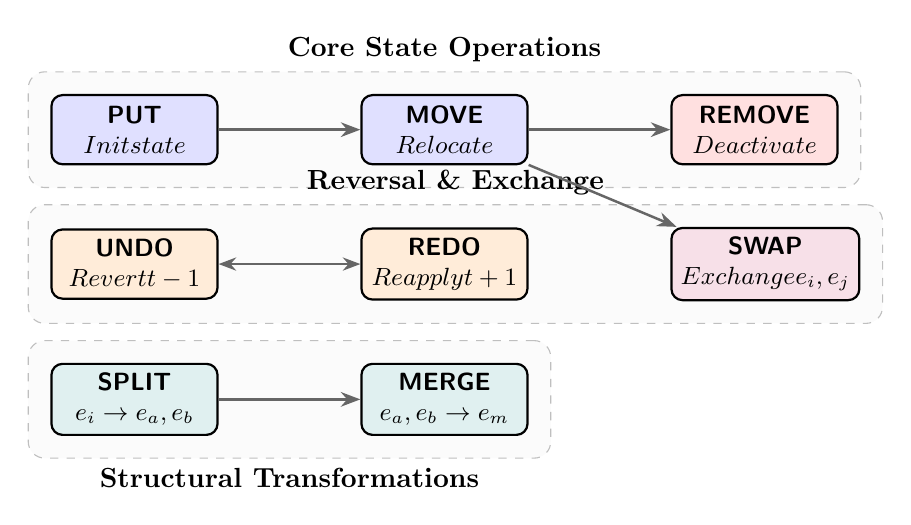
\begin{tikzpicture}[node distance=1.2cm and 1.8cm, auto]
    % Nodes
    \node [block, fill=blue!12] (put) {\textbf{PUT}\\$\text{Init state}$};
    \node [block, fill=blue!12, right=of put] (move) {\textbf{MOVE}\\$\text{Relocate}$};
    \node [block, fill=red!12, right=of move] (remove) {\textbf{REMOVE}\\$\text{Deactivate}$};
    
    \node [block, fill=orange!15, below=0.8cm of put] (undo) {\textbf{UNDO}\\$\text{Revert } t-1$};
    \node [block, fill=orange!15, right=of undo] (redo) {\textbf{REDO}\\$\text{Reapply } t+1$};
    \node [block, fill=purple!12, right=of redo] (swap) {\textbf{SWAP}\\$\text{Exchange } e_i, e_j$};
    
    \node [block, fill=teal!12, below=0.8cm of undo] (split) {\textbf{SPLIT}\\$e_i \rightarrow e_a, e_b$};
    \node [block, fill=teal!12, right=of split] (merge) {\textbf{MERGE}\\$e_a, e_b \rightarrow e_m$};
    
    % Connections
    \draw [arrow] (put) -- (move);
    \draw [arrow] (move) -- (remove);
    \draw [darrow] (undo) -- (redo);
    \draw [arrow] (move) -- (swap);
    \draw [arrow] (split) -- (merge);
    
    % Group containers
    \begin{scope}[on background layer]
        \node [container, fit=(put) (move) (remove), label=above:\textbf{Core State Operations}] {};
        \node [container, fit=(undo) (redo) (swap), label=above:\textbf{Reversal \& Exchange}] {};
        \node [container, fit=(split) (merge), label=below:\textbf{Structural Transformations}] {};
    \end{scope}
\end{tikzpicture}
\caption{DWS-Bench eight-operation vocabulary taxonomy.}
\label{fig:operation-taxonomy}
\end{figure}

\section{Experimental Factors and Structural Control}
Every instance records seven realized factors (Table~\ref{tab:experimental-contract}). Baseline distractor conditions use length-matching controls ($\pm 3$ words) using narrative distractors ($N$) to isolate symbolic updates ($D$) from raw token length ($L$).

\begin{table}[H]
\centering
\small
\renewcommand{\arraystretch}{1.2}
\begin{tabular}{c p{0.45\textwidth} p{0.32\textwidth}}
\toprule
\textbf{Factor} & \textbf{Description} & \textbf{Experimental Role} \\
\midrule
$E$ & Entity count & World state entity load \\
$T$ & Target-relevant update depth & Temporal dependency depth \\
$D$ & State-changing distractor updates & Symbolic state interference \\
$N$ & Narrative-level distractors & Surface text length equalizer \\
$V$ & State revision count & History overwriting pressure \\
$U$ & Total canonical updates & Overall trajectory size \\
$L$ & Rendered word count proxy & Context length diagnostic \\
\bottomrule
\end{tabular}
\caption{DWS-Bench recorded complexity factors.}
\label{tab:experimental-contract}
\end{table}

\begin{figure}[H]
\centering
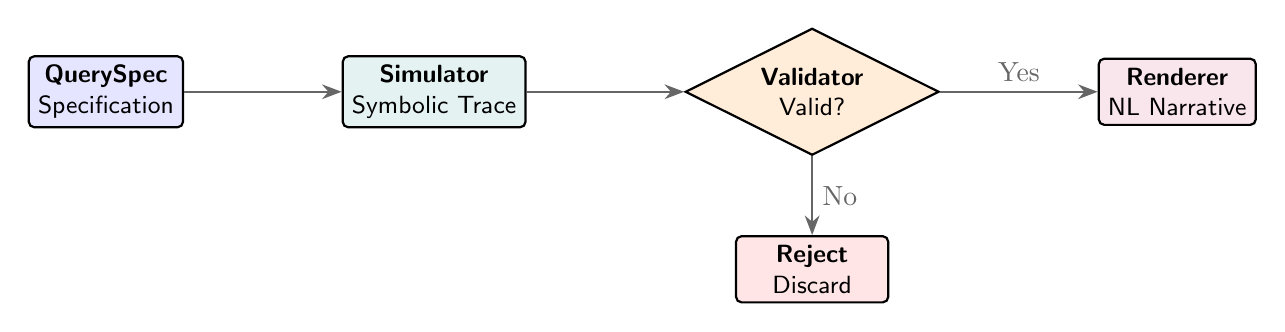
\begin{tikzpicture}[node distance=1.5cm and 2.0cm, auto]
    \node [process, fill=blue!10] (qs) {\textbf{QuerySpec}\\Specification};
    \node [process, fill=teal!10, right=of qs] (sim) {\textbf{Simulator}\\Symbolic Trace};
    \node [decision, right=of sim] (val) {\textbf{Validator}\\Valid?};
    \node [process, fill=purple!10, right=of val] (ren) {\textbf{Renderer}\\NL Narrative};
    \node [process, fill=red!10, below=1.0cm of val] (rej) {\textbf{Reject}\\Discard};
    
    \draw [arrow] (qs) -- (sim);
    \draw [arrow] (sim) -- (val);
    \draw [arrow] (val) -- node [above] {Yes} (ren);
    \draw [arrow] (val) -- node [right] {No} (rej);
\end{tikzpicture}
\caption{DWS-Bench trajectory validation flow.}
\label{fig:validation-flow}
\end{figure}

Ground truth labels are strictly computed from symbolic simulation $S_U$:
\begin{equation}
\mathrm{GroundTruth} = G(S_U, q)
\end{equation}
The natural-language renderer cannot alter symbolic gold labels, preventing ground-truth drift.

% =================================================================
% CHAPTER 5 -- METHODOLOGY
% =================================================================
\chapter{Methodology}

\section{System Architecture}
The DWS-Bench workflow separates symbolic trajectory construction, validation, narrative rendering, and model evaluation into a modular pipeline (Figure~\ref{fig:system-overview}).

\begin{figure}[H]
\centering
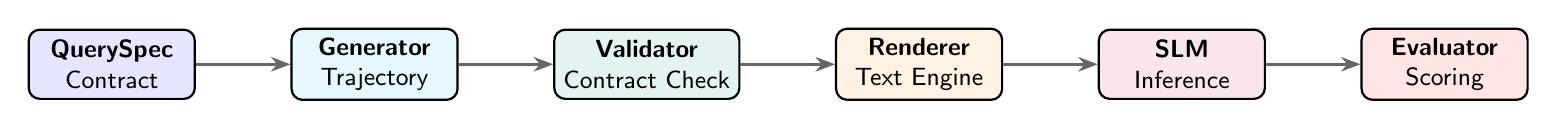
\begin{tikzpicture}[node distance=1.0cm and 1.2cm, auto]
    \node [block, fill=blue!10] (qs) {\textbf{QuerySpec}\\Contract};
    \node [block, fill=cyan!10, right=of qs] (gen) {\textbf{Generator}\\Trajectory};
    \node [block, fill=teal!10, right=of gen] (val) {\textbf{Validator}\\Contract Check};
    \node [block, fill=orange!10, right=of val] (ren) {\textbf{Renderer}\\Text Engine};
    \node [block, fill=purple!10, right=of ren] (slm) {\textbf{SLM}\\Inference};
    \node [block, fill=red!10, right=of slm] (eval) {\textbf{Evaluator}\\Scoring};

    \draw [arrow] (qs) -- (gen);
    \draw [arrow] (gen) -- (val);
    \draw [arrow] (val) -- (ren);
    \draw [arrow] (ren) -- (slm);
    \draw [arrow] (slm) -- (eval);
\end{tikzpicture}
\caption{DWS-Bench system architecture pipeline.}
\label{fig:system-overview}
\end{figure}

\begin{figure}[H]
\centering
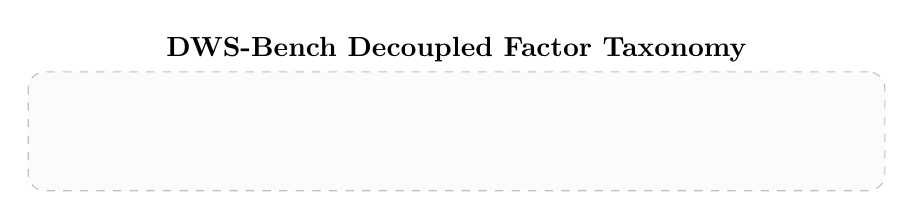
\begin{tikzpicture}[node distance=1.2cm and 1.5cm]
    \node [block, fill=gray!12] (sym) {\textbf{Symbolic State Complexity}\\$(E, T, D, V, U)$};
    \node [block, fill=gray!12, right=of sym] (surf) {\textbf{Surface Rendering Complexity}\\$(N, L)$};
    \node [container, fit=(sym) (surf), label=above:\textbf{DWS-Bench Decoupled Factor Taxonomy}] {};
\end{tikzpicture}
\caption{DWS-Bench factor taxonomy separating state complexity from surface noise.}
\label{fig:factor-taxonomy}
\end{figure}

\section{Evaluation Protocols}
Evaluating models across three Qwen2.5 parameter variants (\mbox{0.5B}, \mbox{3B}, \mbox{7B}) under two prompting regimes (Direct Zero-Shot and Chain-of-Thought).
\begin{itemize}[noitemsep]
    \item \textbf{Final-Answer Accuracy:} String matching normalized state outputs against $S_U$.
    \item \textbf{Step-Wise Accuracy:} Evaluating inferred states $\hat{S}_t$ against symbolic intermediate states $S_t$ at every target update step $t \in \{1, \dots, T\}$.
\end{itemize}

\section{Counterfactual Probe Support}
The repository contains support for constructing counterfactual probes by changing a controlled operation or state transition while preserving the surrounding context as closely as the generator permits. No populated counterfactual probe results are included in the current evaluation artifacts, so this capability is treated as infrastructure for future experiments rather than as an empirical finding in this thesis.

% =================================================================
% CHAPTER 6 -- IMPLEMENTATION
% =================================================================
\chapter{Implementation}

\section{Software Architecture and Status}
The benchmark repository is structured into decoupled Python modules (Table~\ref{tab:implementation}).

\begin{table}[H]
\centering
\small
\begin{tabular}{ll}
\toprule
\textbf{Module} & \textbf{Responsibility} \\
\midrule
\texttt{Contract / QuerySpec} & Defines condition rules and structural constraints. \\
\texttt{Simulator} & Maintains exact symbolic state transitions and history. \\
\texttt{Generator} & Constructs candidate trajectories satisfying QuerySpecs. \\
\texttt{Validator} & Enforces trajectory admissibility and contract rules. \\
\texttt{Renderer} & Translates symbolic steps into natural language. \\
\texttt{Evaluator} & Runs SLM inference and computes step/final metrics. \\
\bottomrule
\end{tabular}
\caption{DWS-Bench implementation architecture.}
\label{tab:implementation}
\end{table}

Table~\ref{tab:implementation-status} summarizes current implementation status.

\begin{table}[H]
\centering
\small
\begin{tabular}{lll}
\toprule
\textbf{Component} & \textbf{Status} & \textbf{Verification Evidence} \\
\midrule
Symbolic Simulator & Completed & Unit tests \& state assertions \\
8-Operation Vocabulary & Completed & Synthetic state unit tests \\
QuerySpec Layer & Completed & Specification contract tests \\
Validator \& Sampler & Completed & Admissibility suite \\
Phase 1 Validation & Completed & Factor distribution analysis \\
Phase 2 Model Suite & Completed & 1,150 frozen instances evaluated \\
Phase 3 Audit & Pilot & Naturalistic reference corpus \\
\bottomrule
\end{tabular}
\caption{Implementation status summary.}
\label{tab:implementation-status}
\end{table}

% =================================================================
% CHAPTER 7 -- RESULTS AND DISCUSSION
% =================================================================
\chapter{Results and Discussion}
\label{chap:results}

\section{Phase 1: Generator Validation}
Phase 1 verified that generated instances meet QuerySpec bounds prior to freezing (Table~\ref{tab:factor-validation}).

\begin{table}[H]
\centering
\small
\begin{tabular}{cccc}
\toprule
\textbf{Factor} & \textbf{Requested Range} & \textbf{Realized Range} & \textbf{Validation Status} \\
\midrule
$E$ & $1$--$5$ & $1$--$5$ & Verified across benchmark \\
$T$ & $2$--$16$ & $2$--$16$ & Realized in depth sweep \\
$D$ & $0$--$16$ & $0$--$16$ & Realized in distractor sweep \\
$N$ & $\{0, 4\}$ & $\{0, 4\}$ & Matched length control \\
$L$ & $<600$ words & 32--312 words & Word-count proxy verified \\
\bottomrule
\end{tabular}
\caption{Phase 1 factor validation summary on frozen benchmark.}
\label{tab:factor-validation}
\end{table}

\section{Phase 2: Benchmark Model Performance}
Table~\ref{tab:model-summary} details overall benchmark performance across all 1,150 frozen instances.

\begin{table}[H]
\centering
\small
\begin{tabular}{lcccc}
\toprule
\textbf{Model} & \textbf{Prompting} & \textbf{Final Accuracy} & \textbf{Step-wise Accuracy} & \textbf{Instances} \\
\midrule
Qwen2.5-0.5B & Direct & 40.87\% & 25.39\% & 1150 \\
Qwen2.5-0.5B & CoT & 0.17\% & -- & 1150 \\
Qwen2.5-3B & Direct & 25.65\% & 24.07\% & 1150 \\
Qwen2.5-3B & CoT & \textbf{49.91\%} & \textbf{2.82\%} & 1150 \\
Qwen2.5-7B & Direct & 11.39\% & -- & 1150 \\
Qwen2.5-7B & CoT & 10.52\% & 23.99\% & 1150 \\
\bottomrule
\end{tabular}
\caption{Overall benchmark performance across evaluated models.}
\label{tab:model-summary}
\end{table}

\begin{figure}[H]
\centering
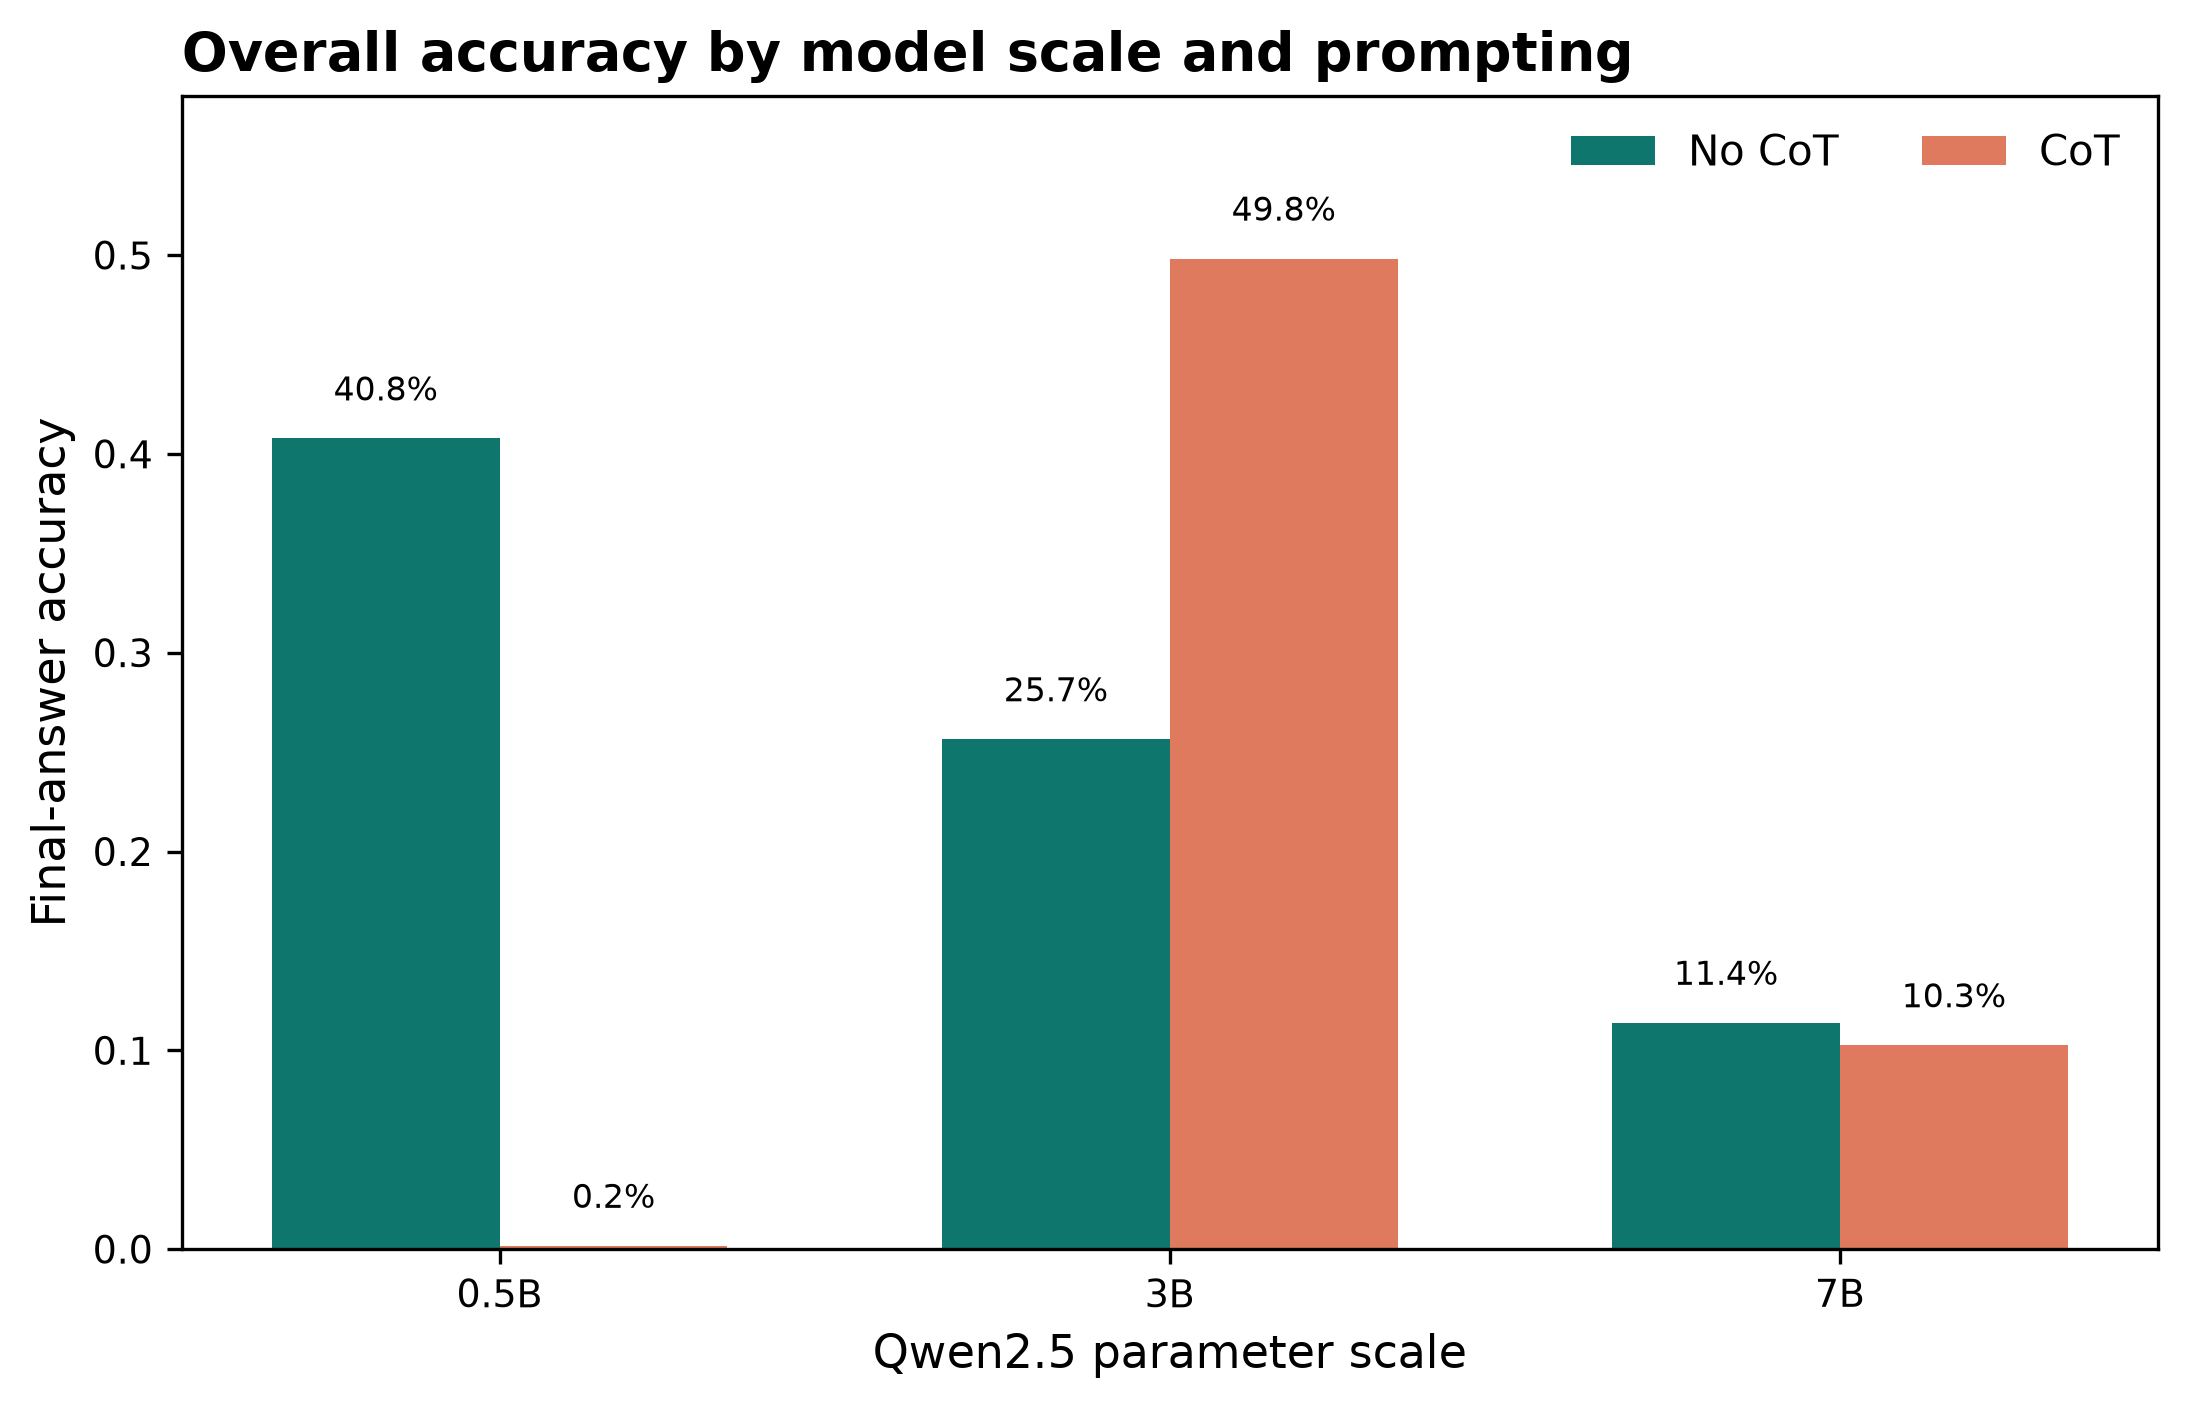
\includegraphics[width=0.85\textwidth]{fig01_overall_model_prompting.png}
\caption{Overall final-answer accuracy across model scales and prompting conditions.}
\label{fig:overall-model-prompting}
\end{figure}

The highest overall accuracy (49.91\%) was achieved by Qwen2.5-3B CoT. However, its step-wise accuracy was only 2.82\%, demonstrating that final answer correctness frequently occurred despite severe intermediate state tracking breakdown. Qwen2.5-0.5B CoT collapsed to 0.17\%, showing CoT prompting can severely degrade performance in ultra-small models.

\section{RQ1: Temporal Depth Results}
Table~\ref{tab:rq1-results} and Figure~\ref{fig:rq1-temporal-depth} present final-answer accuracy as update depth $T$ increases from 2 to 16.

\begin{table}[H]
\centering
\small
\resizebox{\textwidth}{!}{%
\begin{tabular}{lcccccc}
\toprule
\textbf{Model \& Prompt} & \textbf{$T=2$} & \textbf{$T=4$} & \textbf{$T=6$} & \textbf{$T=8$} & \textbf{$T=12$} & \textbf{$T=16$} \\
\midrule
Qwen2.5-0.5B Direct & 100.0\% & 66.0\% & 24.0\% & 22.0\% & 46.0\% & 36.0\% \\
Qwen2.5-0.5B CoT & 0.0\% & 0.0\% & 0.0\% & 0.0\% & 0.0\% & 0.0\% \\
Qwen2.5-3B Direct & 85.0\% & 88.0\% & 84.0\% & 88.0\% & 84.0\% & 78.0\% \\
Qwen2.5-3B CoT & 100.0\% & 100.0\% & 100.0\% & 98.0\% & 98.0\% & 90.0\% \\
Qwen2.5-7B Direct & 6.0\% & 8.0\% & 14.0\% & 10.0\% & 12.0\% & 8.0\% \\
Qwen2.5-7B CoT & 10.0\% & 12.0\% & 10.0\% & 16.0\% & 8.0\% & 6.0\% \\
\bottomrule
\end{tabular}
}%
\caption{Final-answer accuracy by target update depth ($T$) (RQ1).}
\label{tab:rq1-results}
\end{table}

\begin{figure}[H]
\centering
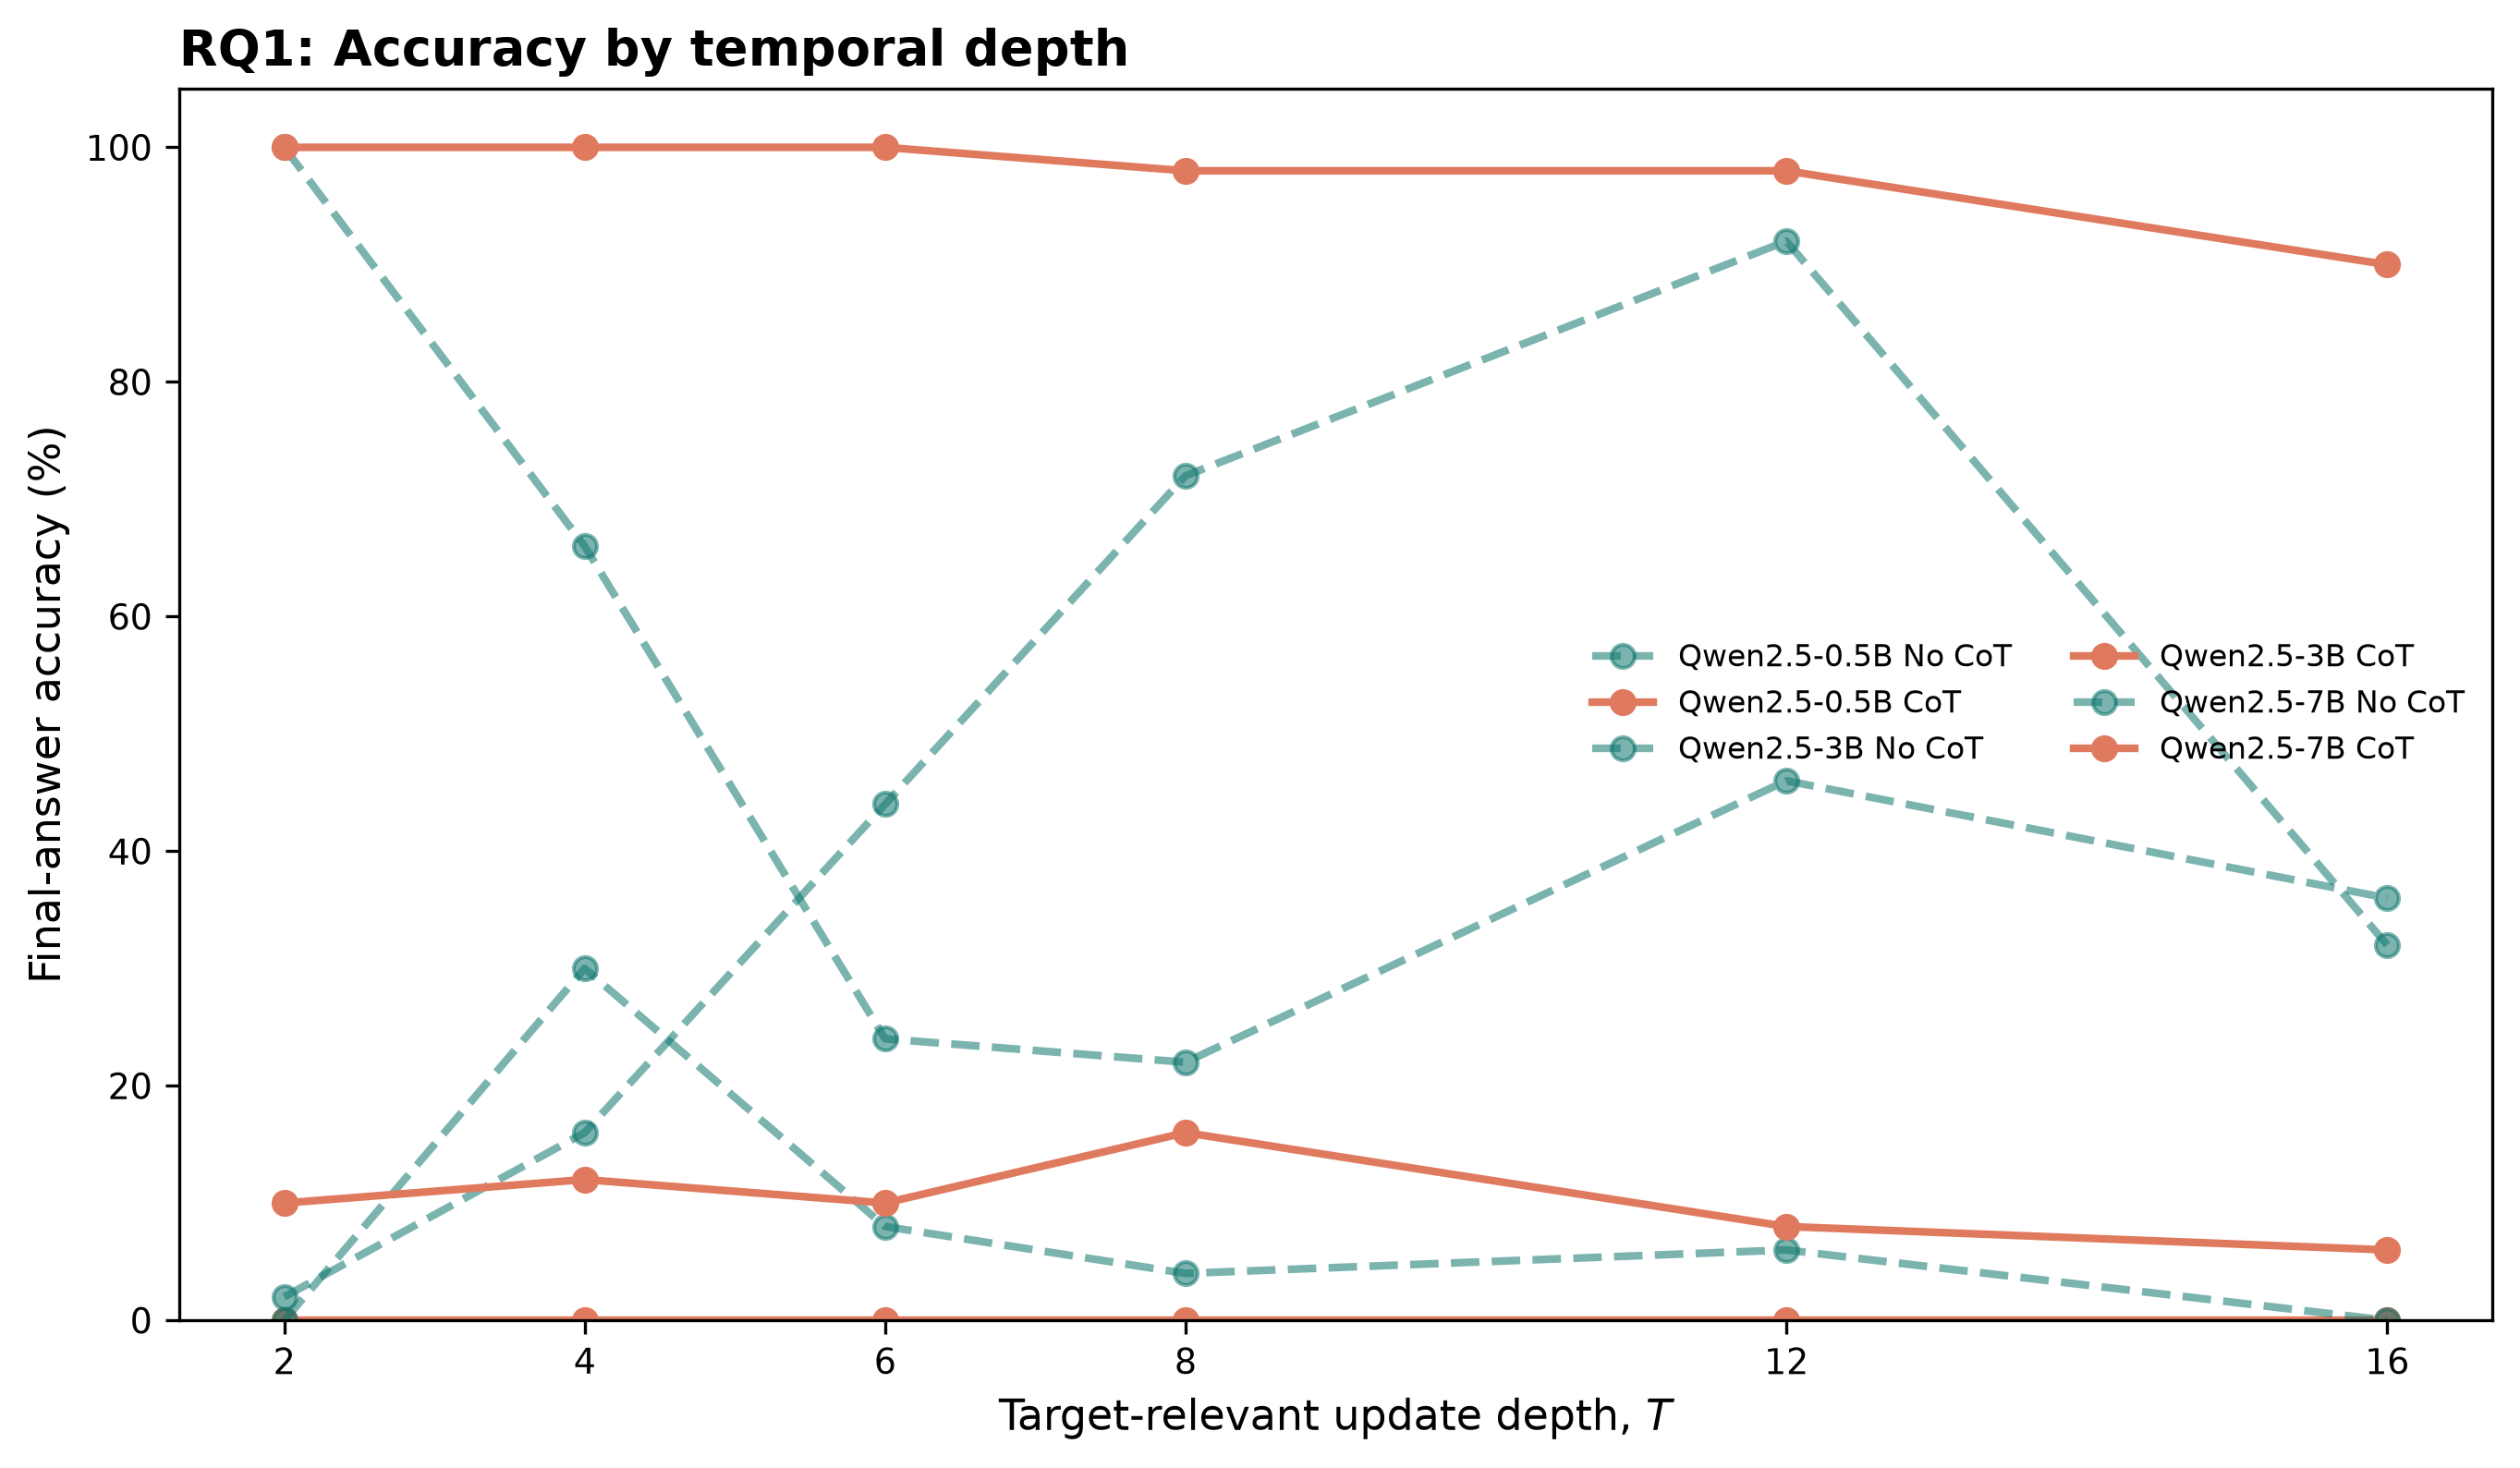
\includegraphics[width=0.85\textwidth]{fig02_rq1_temporal_depth.png}
\caption{RQ1 final accuracy across temporal update depths ($T$).}
\label{fig:rq1-temporal-depth}
\end{figure}

\section{RQ2: State Revision Results}
Table~\ref{tab:rq2-results} reports performance under state overwriting and revision ($V$).

\begin{table}[H]
\centering
\small
\begin{tabular}{lcccc}
\toprule
\textbf{Model \& Prompt} & \textbf{$T=4$} & \textbf{$T=8$} & \textbf{$T=12$} & \textbf{$T=16$} \\
\midrule
Qwen2.5-0.5B Direct & 48.0\% & 40.0\% & 40.0\% & 30.0\% \\
Qwen2.5-0.5B CoT & 0.0\% & 0.0\% & 0.0\% & 0.0\% \\
Qwen2.5-3B Direct & 6.0\% & 10.0\% & 8.0\% & 4.0\% \\
Qwen2.5-3B CoT & 6.0\% & 76.0\% & 2.0\% & 2.0\% \\
Qwen2.5-7B Direct & 4.0\% & 0.0\% & 4.0\% & 0.0\% \\
Qwen2.5-7B CoT & 4.0\% & 14.0\% & 0.0\% & 0.0\% \\
\bottomrule
\end{tabular}
\caption{Final accuracy on state revision sweep (RQ2).}
\label{tab:rq2-results}
\end{table}

\begin{figure}[H]
\centering
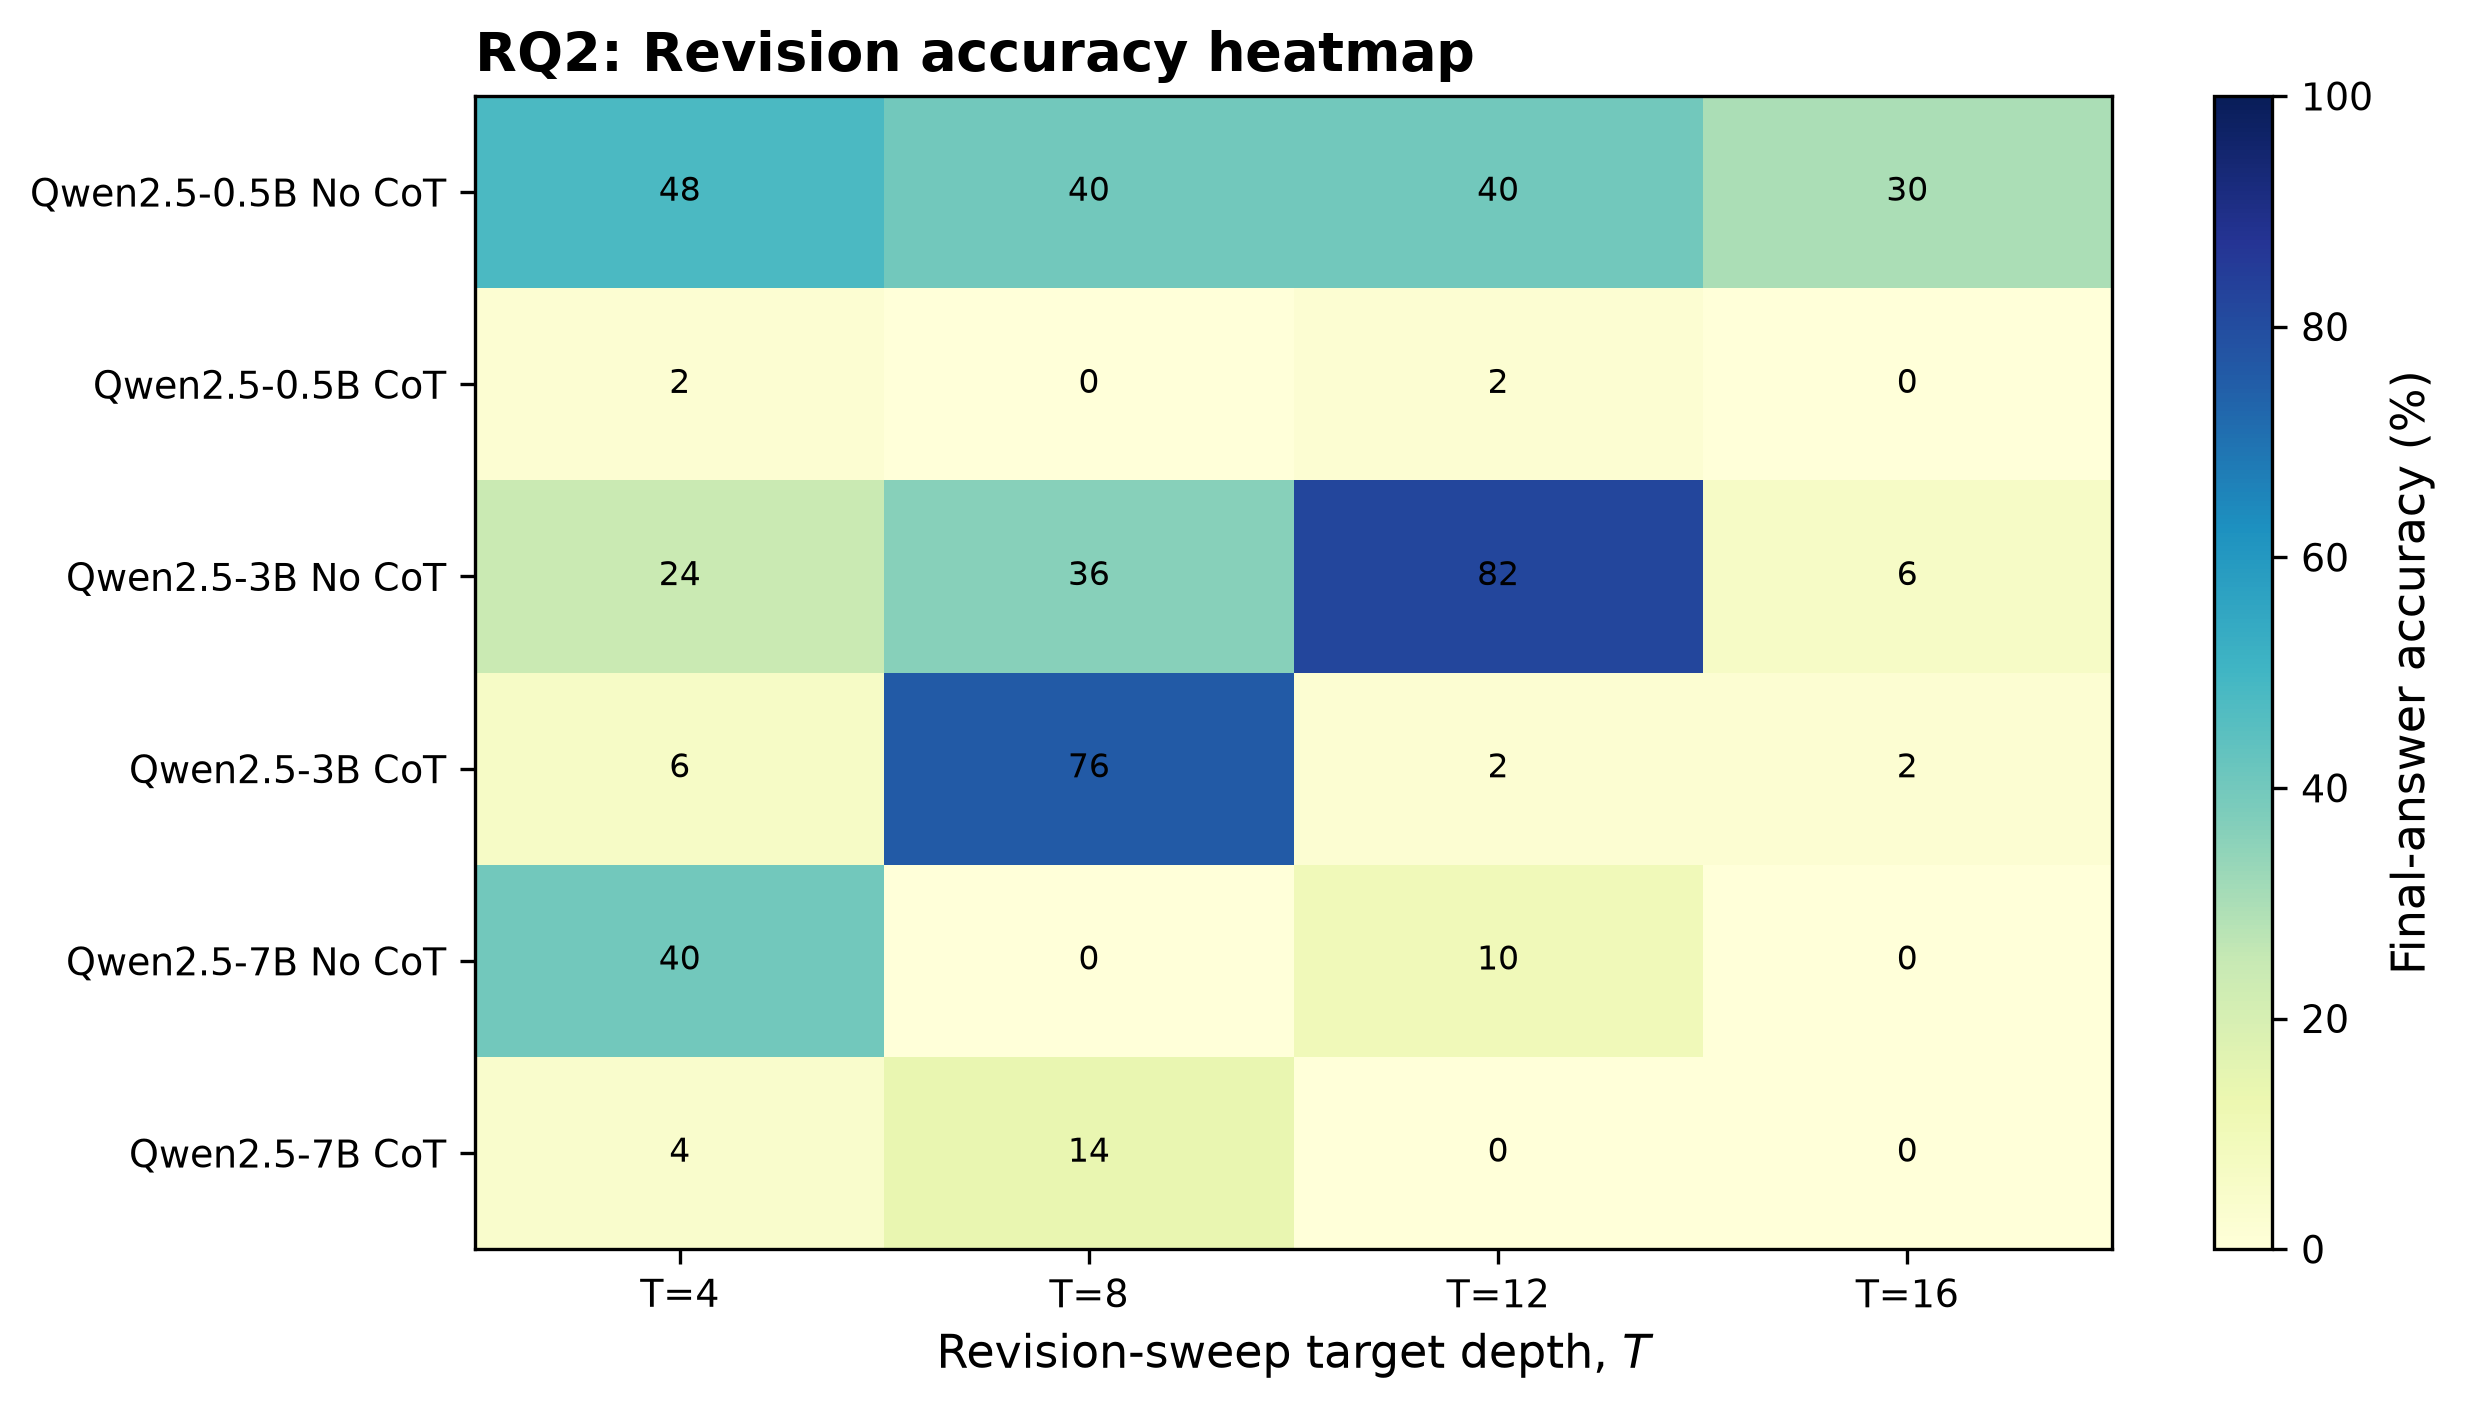
\includegraphics[width=0.85\textwidth]{fig03_rq2_revision_heatmap.png}
\caption{RQ2 accuracy across state revision conditions.}
\label{fig:rq2-revision-heatmap}
\end{figure}

\section{RQ3: Distractor Interference Results}
Table~\ref{tab:rq3-results} details performance under state-changing distractors ($D$).

\begin{table}[H]
\centering
\small
\begin{tabular}{lccc}
\toprule
\textbf{Model \& Prompt} & \textbf{$D=4$} & \textbf{$D=8$} & \textbf{$D=16$} \\
\midrule
Qwen2.5-0.5B Direct & 29.0\% & 38.0\% & 10.0\% \\
Qwen2.5-0.5B CoT & 0.0\% & 0.0\% & 0.0\% \\
Qwen2.5-3B Direct & 18.0\% & 16.0\% & 16.0\% \\
Qwen2.5-3B CoT & 18.7\% & 16.0\% & 16.0\% \\
Qwen2.5-7B Direct & 0.0\% & 0.0\% & 0.0\% \\
Qwen2.5-7B CoT & 7.0\% & 36.0\% & 52.0\% \\
\bottomrule
\end{tabular}
\caption{Final accuracy on distractor sweep (RQ3).}
\label{tab:rq3-results}
\end{table}

\begin{figure}[H]
\centering
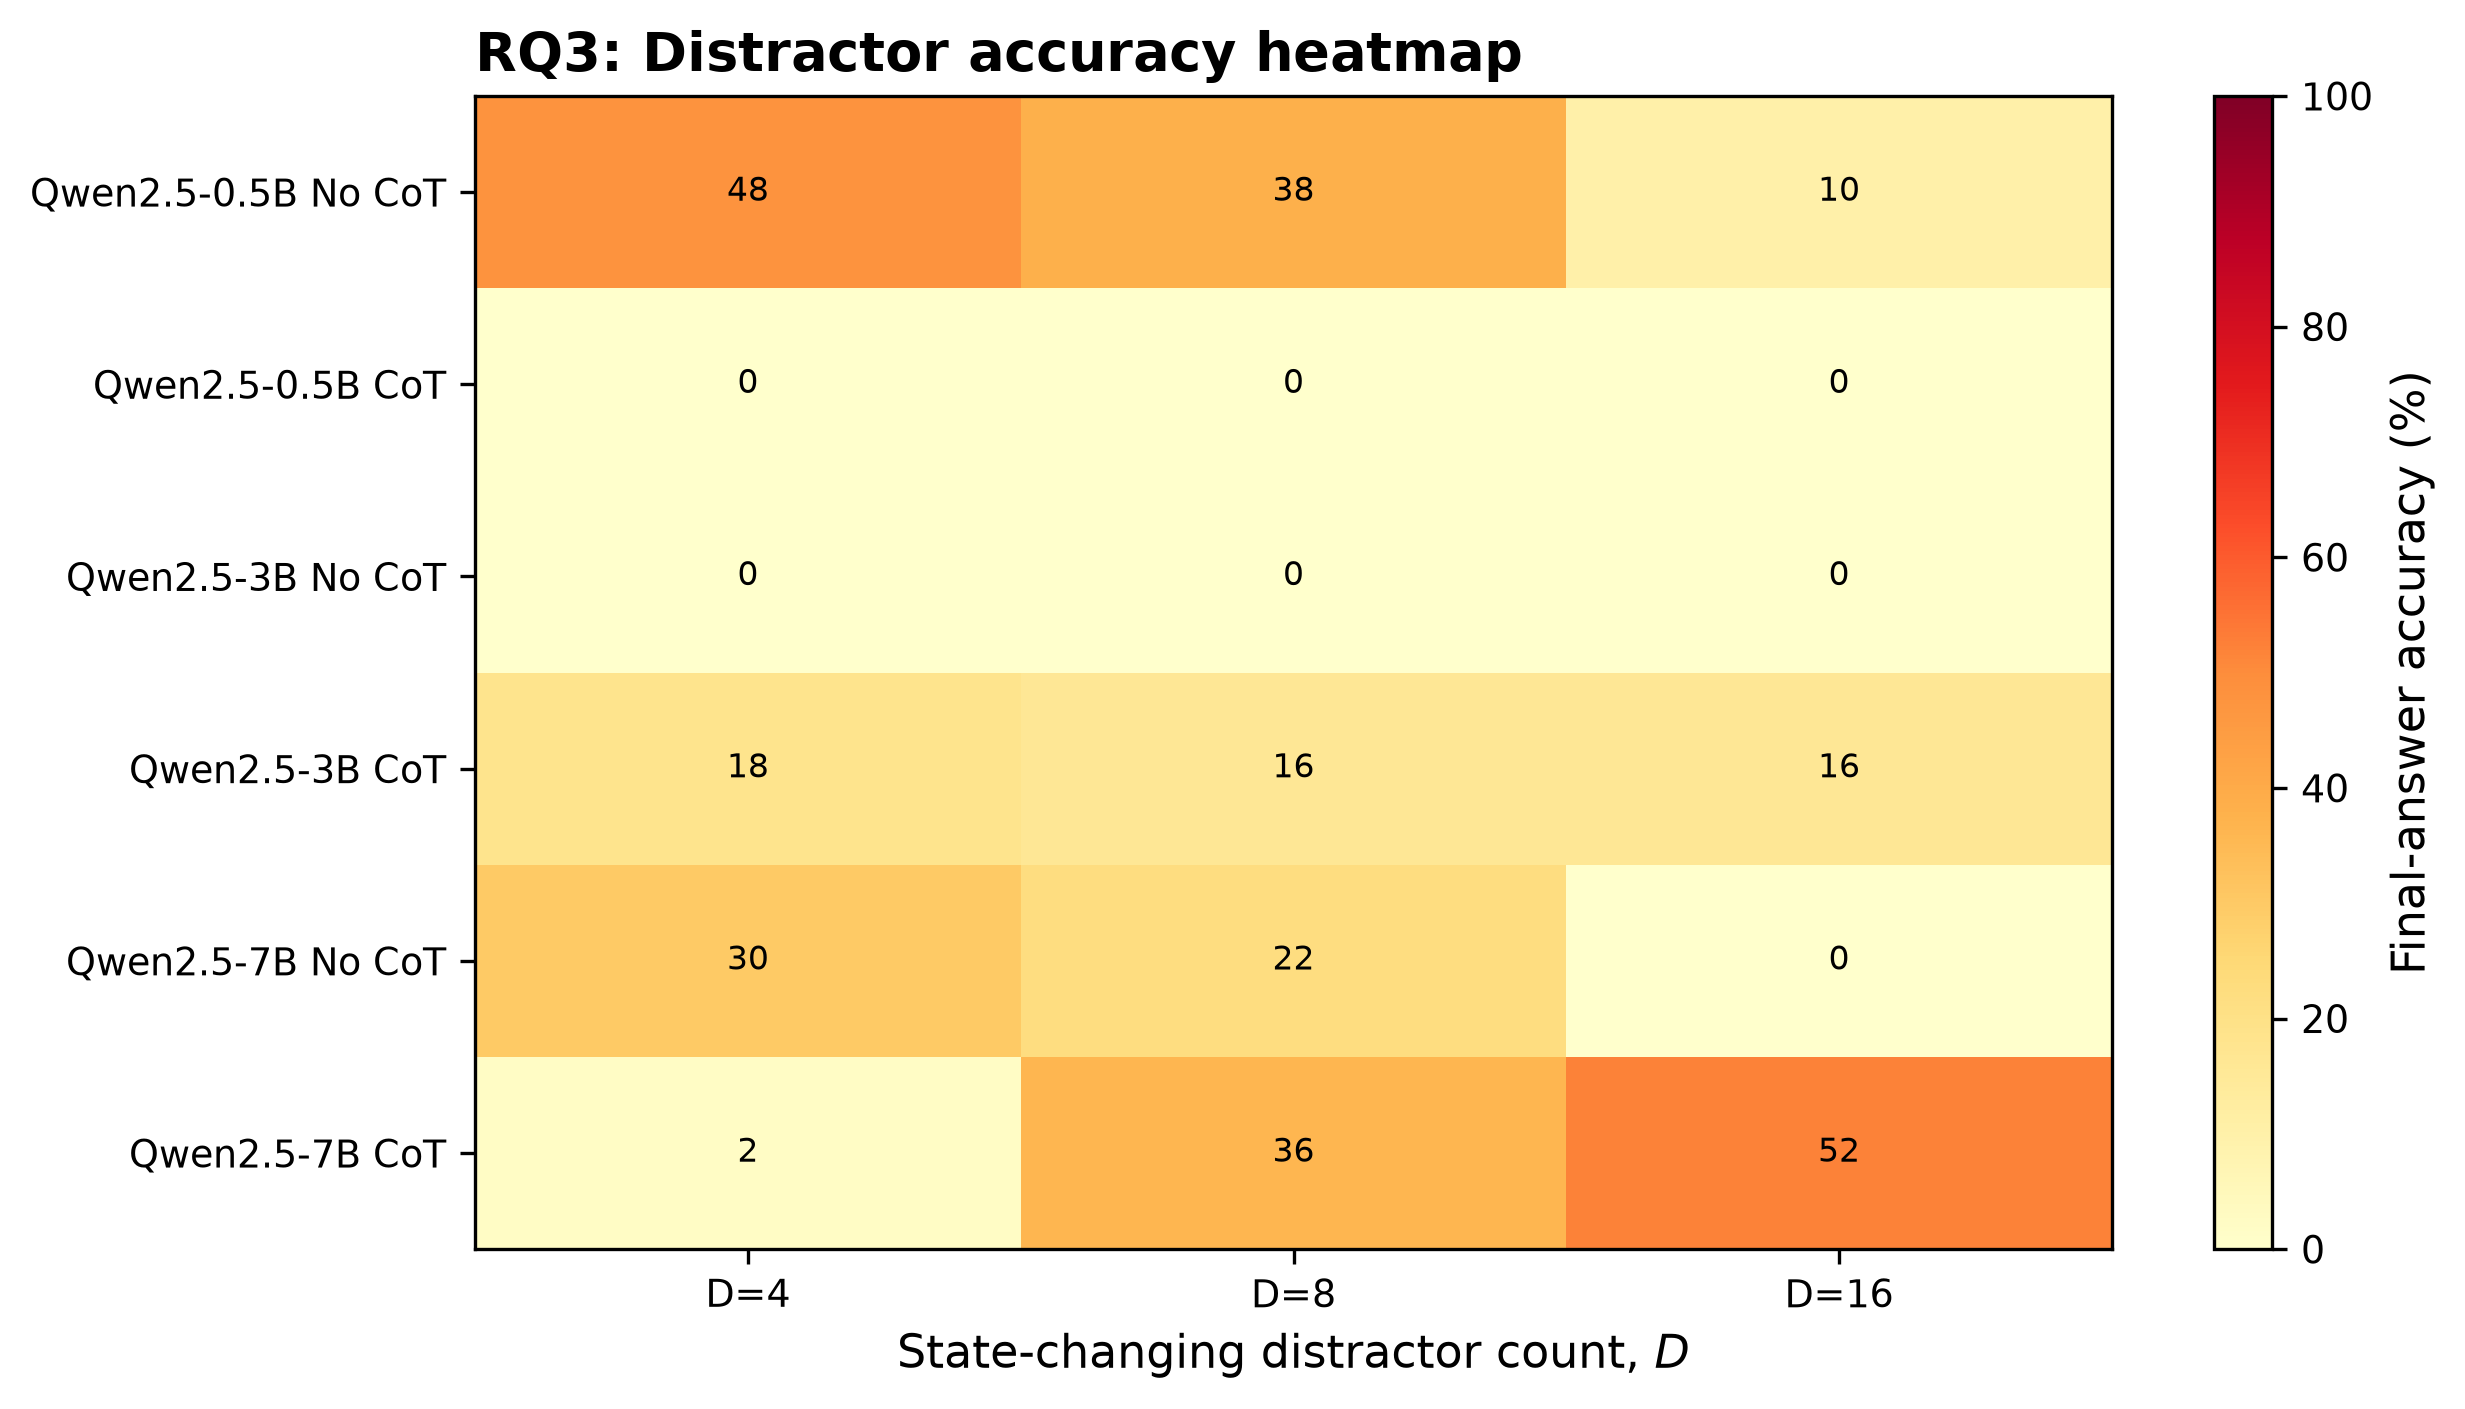
\includegraphics[width=0.85\textwidth]{fig04_rq3_distractor_heatmap.png}
\caption{RQ3 accuracy across state-changing distractor counts.}
\label{fig:rq3-distractor-heatmap}
\end{figure}

\section{RQ4: Entity Load Status}
Entity load sweeps ($E \in \{2,3,4,5\}$) were generated in the benchmark, but evaluation summaries remain pending at the model output level.

\section{RQ5: Structural Operation Pilot Results}
Table~\ref{tab:rq5-results} presents accuracy across five complex operation families (250 instances). Realized factors must be reported: the \texttt{split\_chain} records realize $T_{\mathrm{actual}}=7$ and $D_{\mathrm{actual}}=1$, while the available records for the other four pilot families realize $T_{\mathrm{actual}}=8$ in the frozen data. Because the split family has a different realized target depth, these family comparisons should be interpreted descriptively rather than as perfectly matched causal contrasts.

\begin{table}[H]
\centering
\small
\begin{tabular}{lccccc}
\toprule
\textbf{Model \& Prompt} & \textbf{Split} & \textbf{Merge} & \textbf{Swap} & \textbf{Undo} & \textbf{Undo-Redo} \\
\midrule
Qwen2.5-0.5B Direct & 12.0\% & 68.0\% & 56.0\% & 60.0\% & 68.0\% \\
Qwen2.5-0.5B CoT & 0.0\% & 0.0\% & 0.0\% & 0.0\% & 0.0\% \\
Qwen2.5-3B Direct & 8.0\% & 18.0\% & 20.0\% & 58.0\% & 80.0\% \\
Qwen2.5-3B CoT & 66.0\% & 92.0\% & 18.0\% & 92.0\% & 64.0\% \\
Qwen2.5-7B Direct & 0.0\% & 0.0\% & 8.0\% & 0.0\% & 0.0\% \\
Qwen2.5-7B CoT & 8.0\% & 6.0\% & 6.0\% & 2.0\% & 4.0\% \\
\bottomrule
\end{tabular}
\caption{Final accuracy on structural operation families (RQ5).}
\label{tab:rq5-results}
\end{table}

\begin{figure}[H]
\centering
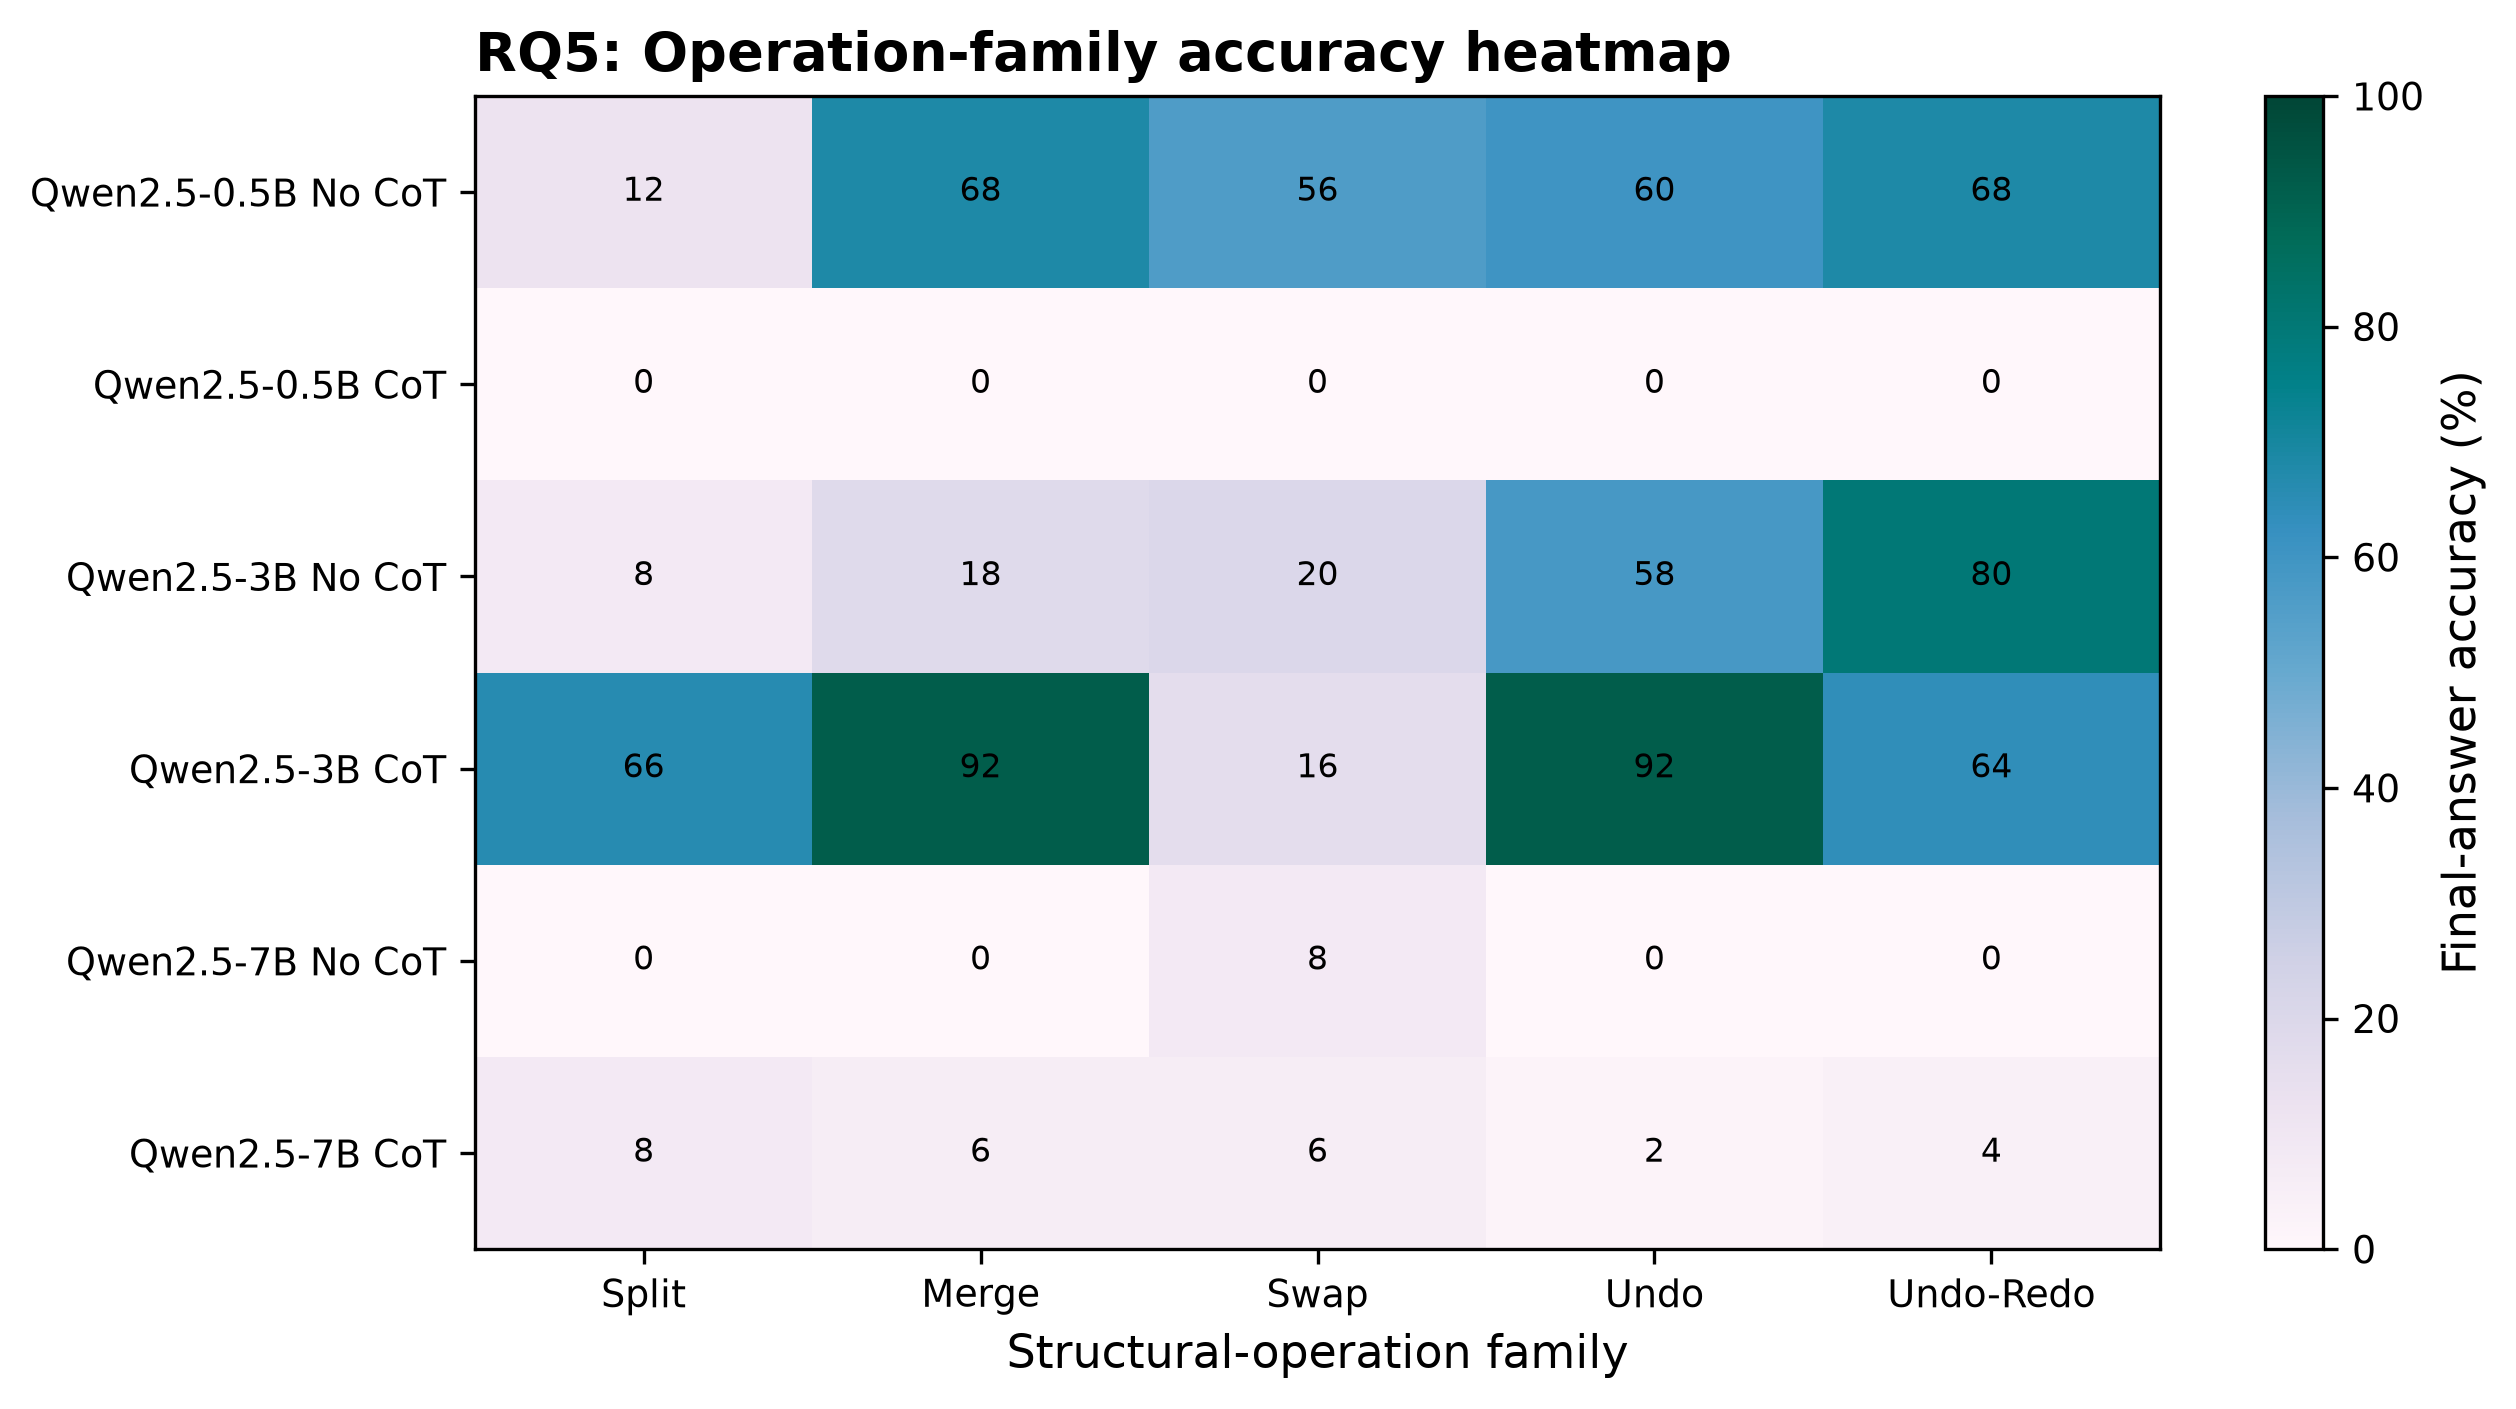
\includegraphics[width=0.85\textwidth]{fig06_rq5_operation_heatmap.png}
\caption{RQ5 accuracy across structural operation families.}
\label{fig:rq5-operation-heatmap}
\end{figure}

\section{Step-Wise vs Final-Answer Error Dynamics}
Figure~\ref{fig:final-vs-stepwise} compares final answer versus step-wise trajectory accuracy.

\begin{figure}[H]
\centering
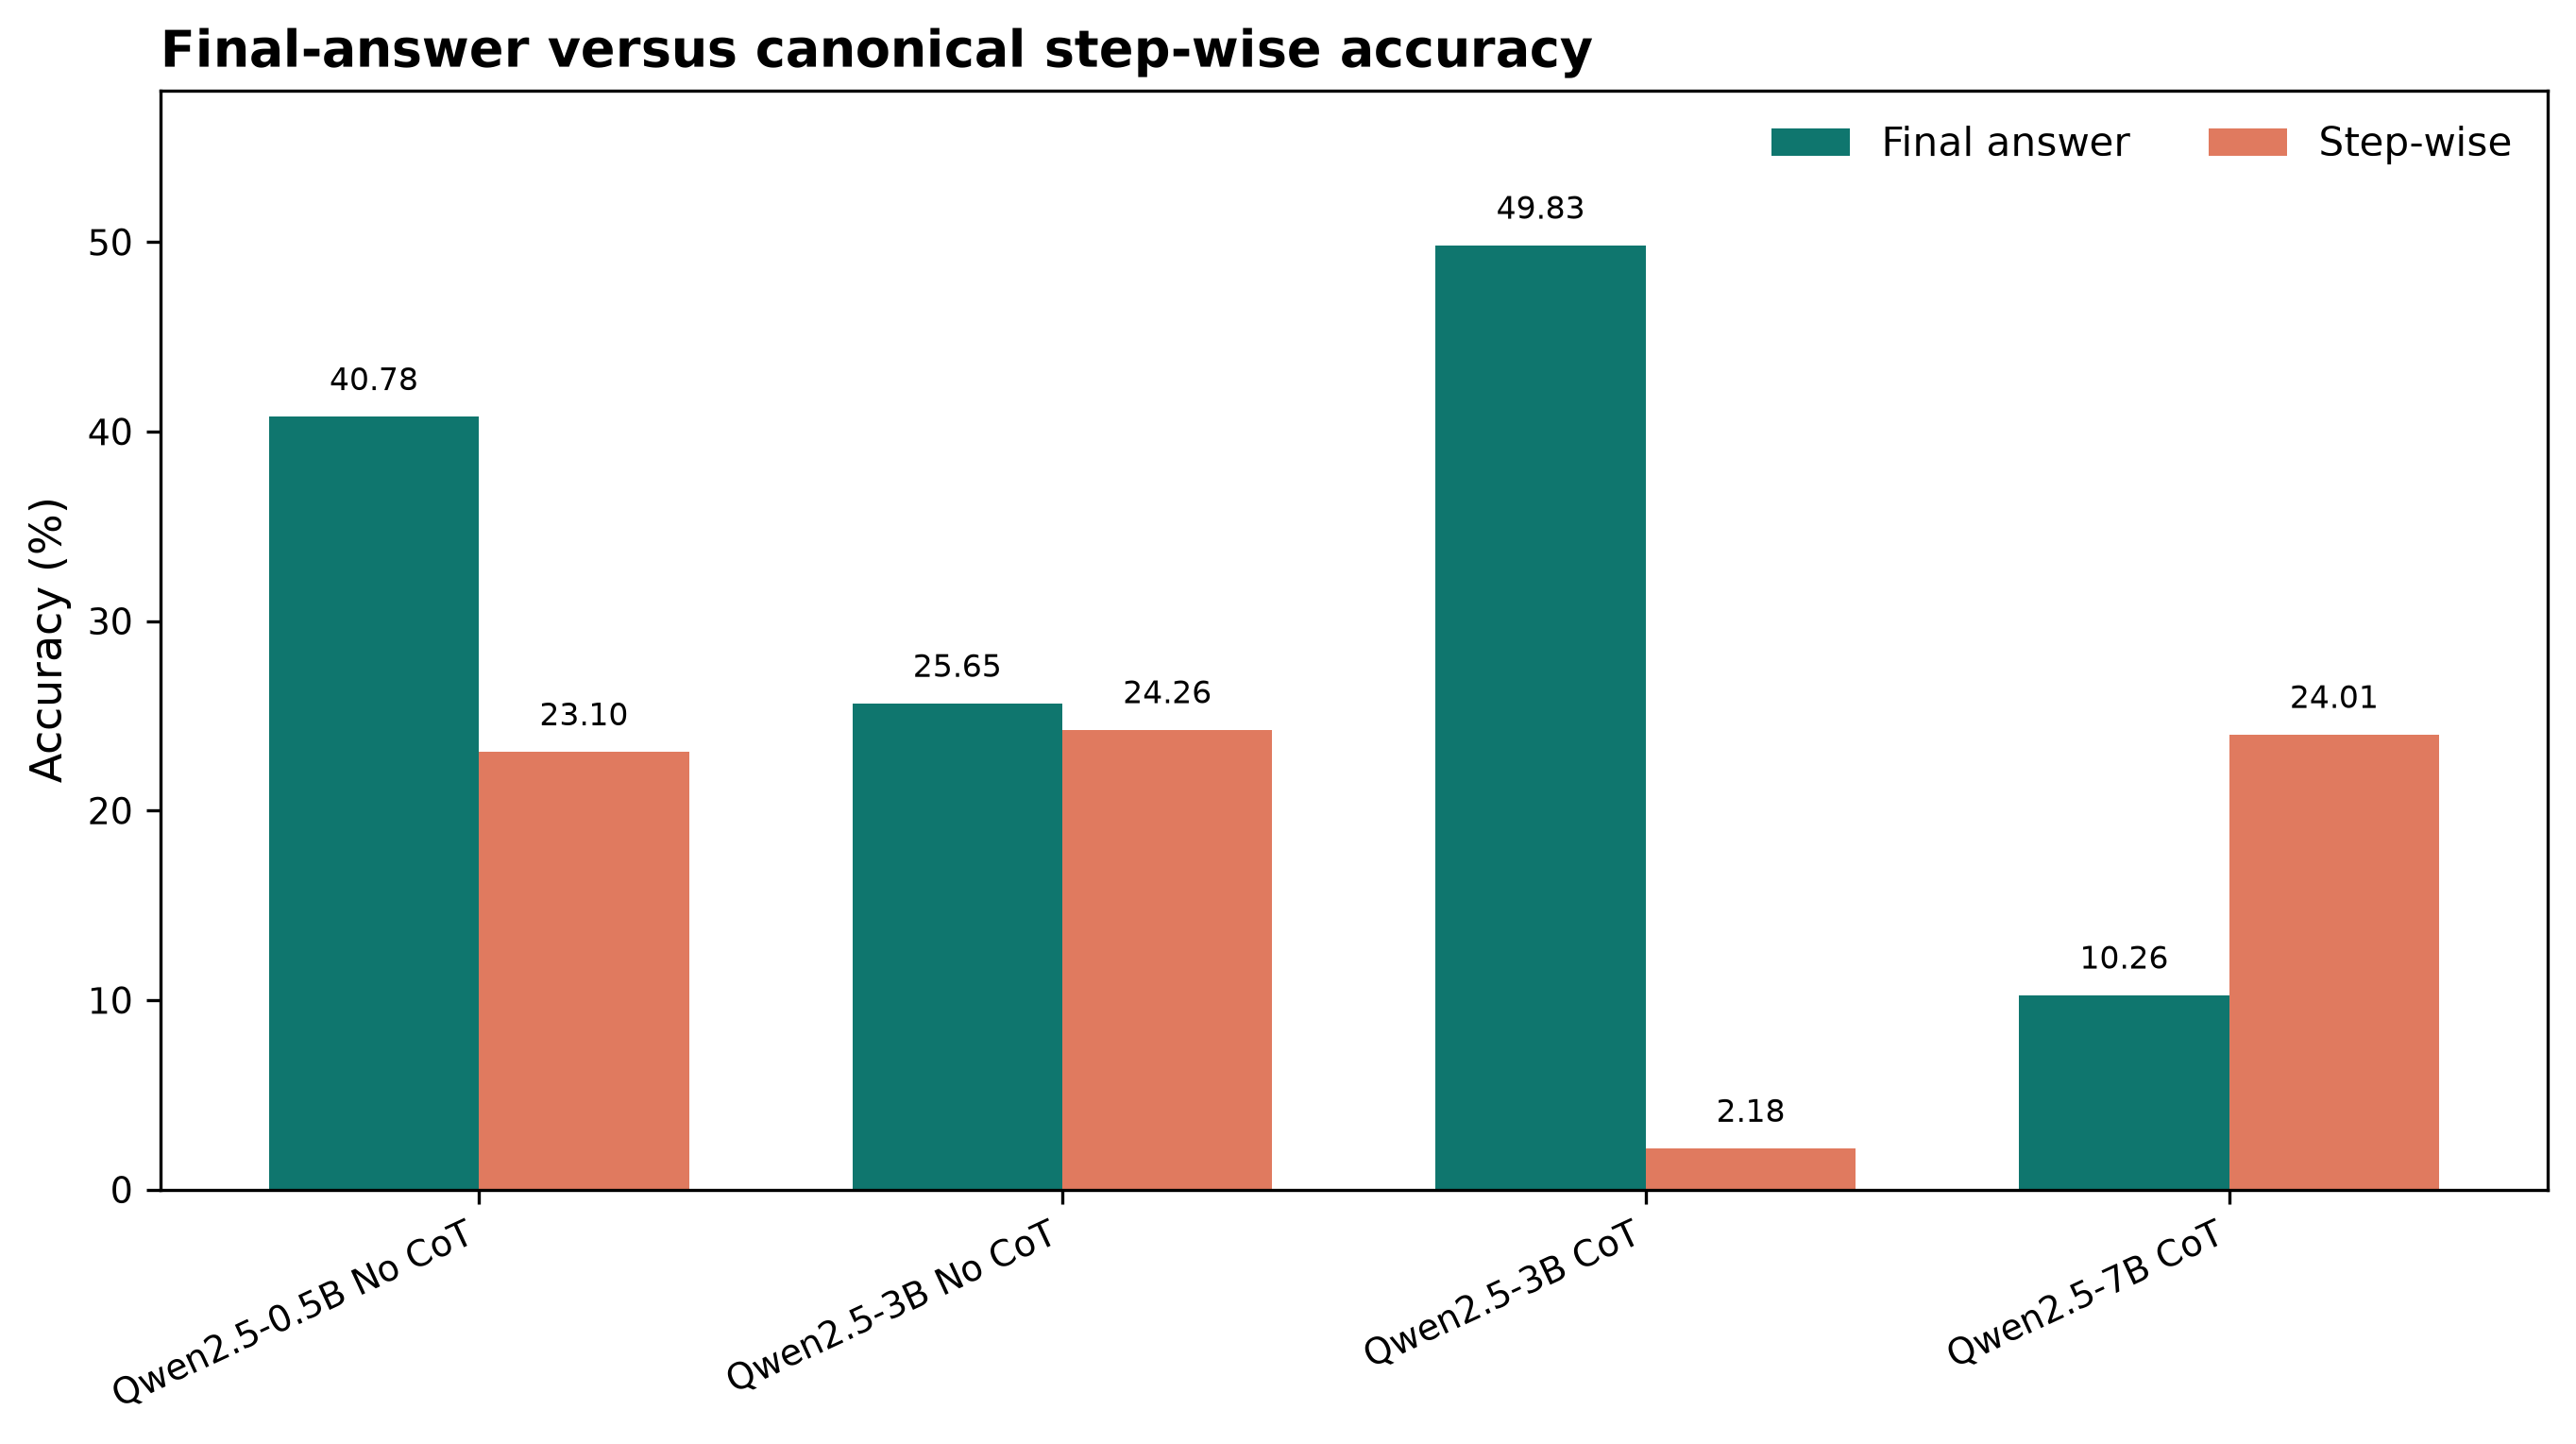
\includegraphics[width=0.85\textwidth]{fig05_final_vs_stepwise.png}
\caption{Final-answer versus step-wise accuracy comparison.}
\label{fig:final-vs-stepwise}
\end{figure}

The stark discrepancy for Qwen2.5-3B CoT (49.91\% final vs. 2.82\% step-wise) indicates that while CoT helps retrieve final answers, it fails to maintain intermediate state accuracy.

\section{Research Question Findings Summary}
Table~\ref{tab:rq-summary} synthesizes key empirical conclusions across research questions.

\begin{table}[H]
\centering
\small
\begin{tabular}{p{0.12\textwidth}p{0.82\textwidth}}
\toprule
\textbf{RQ} & \textbf{Empirical Summary} \\
\midrule
RQ1 & Temporal depth causes non-monotonic degradation; 3B CoT maintains >90\% accuracy through $T=16$, whereas 0.5B Direct drops to 24\% at $T=6$. \\
RQ2 & State revision induces severe failure; 3B CoT drops to 2.0\% at $T=12, 16$. \\
RQ3 & Distractor updates degrade small model accuracy sharply (0.5B drops from 29\% to 10\%). \\
RQ4 & Entity load instances generated; model evaluation output pending. \\
RQ5 & Structural operations display high variance; \texttt{MERGE} and \texttt{UNDO} reach 92\% under 3B CoT, while \texttt{SWAP} remains low (18\%). \\
\bottomrule
\end{tabular}
\caption{Summary of empirical findings across RQs.}
\label{tab:rq-summary}
\end{table}

% =================================================================
% CHAPTER 8 -- ETHICS & SUSTAINABILITY
% =================================================================
\chapter{Ethical, Social, and Environmental Considerations}

\section{Data Integrity and Research Ethics}
DWS-Bench strictly generates synthetic evaluation instances from deterministic symbolic traces. Symbolic labels are computed independently of natural-language text generation, preventing label hallucination. Evaluation protocols report all benchmark slices without selectively filtering low-performing conditions.

\section{Social Accessibility and Environmental Impact}
Small Language Models enable accessible deployment on localized edge devices. Evaluating efficiency vs. reasoning accuracy assists resource-constrained institutions. While model evaluations consume power, evaluating sub-10B parameter models requires significantly less compute than frontier multi-billion parameter evaluations.

% =================================================================
% CHAPTER 9 -- LIMITATIONS
% =================================================================
\chapter{Challenges and Limitations}

\begin{enumerate}[noitemsep]
    \item \textbf{Residual Confounding:} Length-matching ($\pm 3$ words) reduces length confounding but does not eliminate all token-level variances.
    \item \textbf{Synthetic Domain Transfer:} Synthetic text provides clean experimental control but lacks natural language ambiguity.
    \item \textbf{Operation Vocabulary Limits:} The eight operations do not cover spatial topology or containment relations.
    \item \textbf{Model Architecture Scope:} Evaluation focuses on Qwen2.5 instruction-tuned models; results may vary for other architecture families.
\end{enumerate}

% =================================================================
% CHAPTER 10 -- CONCLUSION
% =================================================================
\chapter{Conclusion and Future Work}

\section{Conclusion}
This report introduced \textbf{DWS-Bench}, a controlled benchmark framework isolating dynamic world-state reasoning in Small Language Models. By decoupling symbolic world state updates from natural language rendering, DWS-Bench provides deterministic ground truth across eight canonical operations. Evaluation of Qwen2.5 models revealed that reasoning performance is highly non-monotonic, and that high final-answer accuracy (49.91\% in 3B CoT) can mask severe intermediate trajectory failure (2.82\% step-wise accuracy).

\section{Future Work}
Future extensions include:
\begin{enumerate}[noitemsep]
    \item Broader query types and multi-object questions;
    \item Containment, ownership, and additional relational state representations;
    \item Richer multi-hop and multi-entity reasoning;
    \item Longer and more varied dependency structures;
    \item Broader model and parameter-scale coverage;
    \item Representation-level and mechanistic analysis of state tracking;
    \item Additional naturalistic datasets and transfer settings;
    \item Improved statistical controls for residual context-length confounding;
    \item Expanded trajectory families and operation semantics.
\end{enumerate}

% =================================================================
% APPENDICES
% =================================================================
\begin{appendices}

\chapter{Weekly Meeting Summaries}
Table~\ref{tab:weekly-summary} records weekly progress, decisions, and planned work, reconstructed from the team's WhatsApp group log (``Batch 22 -- Thesis group'').

\begingroup
\small
\begin{longtable}{@{}p{0.04\textwidth}p{0.10\textwidth}p{0.22\textwidth}p{0.22\textwidth}p{0.22\textwidth}@{}}
\caption{Weekly meeting summaries and project progress.} \label{tab:weekly-summary}\\
\hline
\textbf{No.} & \textbf{Date} & \textbf{Progress / Contribution} & \textbf{Decision / Discussion} & \textbf{Next Plan} \\
\hline
\endfirsthead

\multicolumn{5}{l}{\small\textit{(continued from previous page)}} \\
\hline
\textbf{No.} & \textbf{Date} & \textbf{Progress / Contribution} & \textbf{Decision / Discussion} & \textbf{Next Plan} \\
\hline
\endhead

\hline
\multicolumn{5}{r}{\small\textit{(continued on next page)}} \\
\endfoot

\hline
\endlastfoot

1 & 14--18 May 2026 & Started literature review on LLM interpretability and concept representations. Set up the thesis GitHub repository. & Discussed LRH, CRH, steering vectors, and their limitations. & Read background papers and prepare for supervisor discussion. \\
\hline
2 & 20--22 May 2026 & Reviewed additional papers shared by the supervisor. & Discussed the need to understand the papers before selecting a research direction. & Review the remaining papers and identify possible research gaps. \\
\hline
3 & 28 May--02 June 2026 & Continued literature review; supervisor shared work on LLM working memory. & Working memory and reasoning became potential areas of interest. & Continue literature review and arrange the next meeting. \\
\hline
4 & 03--05 June 2026 & Coordinated and attended a supervisor meeting. & Discussed the team's progress and ongoing literature exploration. & Continue narrowing down the research direction. \\
\hline
5 & 10--12 June 2026 & Progress was temporarily limited due to ML coursework and quizzes. & Meeting was postponed with supervisor approval. & Resume thesis work after academic deadlines. \\
\hline
6 & 14--17 June 2026 & Prepared to discuss accumulated literature findings with the supervisor. & Meeting was arranged to review progress and possible research directions. & Present findings and identify a feasible research problem. \\
\hline
7 & 14--15 July 2026 & Converged toward SLM reasoning and state-tracking evaluation. Draft proposal was shared. & Identified a possible gap in multi-parameter evaluation of SLM state tracking. Proposed adapting Kim \& Schuster's (ACL 2023) entity-tracking generator. & Refine the research gap and benchmark design. \\
\hline
8 & 17--23 July 2026 & Continued refining the SLM state-tracking proposal after a postponed meeting. & Supervisor meeting was rescheduled. & Discuss the benchmark and research gap in detail. \\
\hline
9 & 23--31 July 2026 & Refined the project toward a controlled dynamic world-state benchmark. & Discussed using a deterministic simulator and controllable task parameters. & Formalize the variables and begin implementation. \\
\hline
10 & 03 August 2026 & Continued literature review and benchmark methodology development. & Focused on isolating different sources of difficulty in SLM state tracking. & Implement the deterministic state-generation and validation pipeline. \\
\hline
11 & 09--14 August 2026 & Formalized the symbolic-simulator-first approach and experimental variables. & Ground truth should be generated independently from natural-language rendering. & Test alternative rendering approaches on a small pilot set. \\
\hline
12 & 15 August 2026 & Discussed deterministic question generation versus LLM-based paraphrasing. Reviewed related task formulations such as LinearWorld, HandSwap, and Lights. & Supervisor recommended testing both approaches at small scale. Team considered deterministic variation preferable due to lower risk of ground-truth drift. & Run a small comparison and finalize the rendering strategy. \\
\hline
\end{longtable}
\endgroup

\chapter{Implementation and Artifacts}

\section{Repository Architecture}
Table~\ref{tab:repository-components} lists key repository modules.

\begin{table}[H]
\centering
\small
\begin{tabular}{ll}
\toprule
\textbf{Component} & \textbf{Module Scope} \\
\midrule
\texttt{Contract} & Specification of QuerySpecs and complexity rules \\
\texttt{Generator} & Candidate symbolic trajectory generation \\
\texttt{Validator} & Admissibility and ground-truth verification \\
\texttt{Renderer} & Natural language narrative translation \\
\texttt{Evaluator} & Model inference and metric computation \\
\bottomrule
\end{tabular}
\caption{Repository structure overview.}
\label{tab:repository-components}
\end{table}

\section{Technical Contribution Matrix}
Table~\ref{tab:technical-contributions} details individual contributions.

\begin{table}[H]
\centering
\small
\renewcommand{\arraystretch}{1.4}
\begin{tabular}{|p{0.22\textwidth}|p{0.12\textwidth}|p{0.50\textwidth}|}
\hline
\textbf{Member} & \textbf{PR ID} & \textbf{Technical Contribution} \\
\hline
MD. Mahiul Kabir & -- & Symbolic World Simulator and Experimental Contract implementation. \\
\hline
MD. Mahiul Kabir & -- & Repository artifact documentation and implementation validation. \\
\hline
Rahatut Tahrim Mounota & -- & Trajectory Generator and Validation Logic implementation. \\
\hline
Rahatut Tahrim Mounota & -- & Benchmark validation and result-aggregation support. \\
\hline
Nayeemul Hasan Prince & -- & Natural-Language Renderer and Prompt Generation. \\
\hline
Nayeemul Hasan Prince & -- & Report synthesis and evidence-alignment review. \\
\hline
\end{tabular}
\caption{Technical contribution matrix.}
\label{tab:technical-contributions}
\end{table}

\section{GitHub Metrics and Verification}
Tables~\ref{tab:github-metrics} and \ref{tab:pr-verification} document repository activity.

\begin{table}[H]
\centering
\small
\begin{tabular}{p{0.28\textwidth}p{0.17\textwidth}p{0.17\textwidth}p{0.17\textwidth}}
\toprule
\textbf{Member} & \textbf{Commits} & \textbf{Additions} & \textbf{Deletions} \\
\midrule
MD. Mahiul Kabir & 2 & 2,728 & 26 \\
Rahatut Tahrim Mounota & 13 & 787,654 & 6,457 \\
Nayeemul Hasan Prince & 2 & 6,567 & 6,823 \\
\midrule
\textbf{Total} & 17 & 796,949 & 13,306 \\
\bottomrule
\end{tabular}
\caption{GitHub contribution metrics.}
\label{tab:github-metrics}
\end{table}

\begin{table}[H]
\centering
\small
\begin{tabular}{p{0.28\textwidth}p{0.27\textwidth}p{0.27\textwidth}}
\toprule
\textbf{Member} & \textbf{PR 1} & \textbf{PR 2} \\
\midrule
MD. Mahiul Kabir & -- & -- \\
Rahatut Tahrim Mounota & -- & -- \\
Nayeemul Hasan Prince & -- & -- \\
\bottomrule
\end{tabular}
\caption{Pull Request verification matrix.}
\label{tab:pr-verification}
\end{table}

\chapter{Final Compliance Audit}
Table~\ref{tab:final-audit} completes the final submission compliance checklist.

\begin{table}[H]
\centering
\small
\renewcommand{\arraystretch}{1.4}
\begin{tabular}{|p{0.12\textwidth}|p{0.62\textwidth}|p{0.12\textwidth}|}
\hline
\textbf{State} & \textbf{Requirement} & \textbf{Status} \\
\hline
\textbf{Done} & Chapters 1--10 contain complete methodological and empirical content. & Completed \\
\hline
\textbf{Done} & Phase 1 generator validation and factor-distribution analysis completed. & Completed \\
\hline
\textbf{Done} & Realized factor associations have been inspected before benchmark freezing. & Completed \\
\hline
\textbf{Done} & Frozen benchmark datasets are used for Phase 2 evaluation. & Completed \\
\hline
\textbf{Done} & Three target SLMs have been evaluated under the fixed protocol. & Completed \\
\hline
\textbf{Done} & Final-answer and step-wise accuracy are reported. & Completed \\
\hline
\textbf{Done} & RQ1--RQ3 results and interpretations are reported. & Completed \\
\hline
\textbf{Open} & RQ4 evaluation remains pending. & Pending \\
\hline
\textbf{Done} & RQ5 structural-operation families are generated, validated, and evaluated within the core benchmark. & Completed \\
\hline
\textbf{Done} & Performance-degradation and error-dynamics analyses are reported. & Completed \\
\hline
\textbf{Open} & Naturalistic reference audit is documented as a secondary analysis. & Pilot / Descriptive \\
\hline
\textbf{Done} & Symbolic ground truth is independent of the natural-language renderer. & Completed \\
\hline
\textbf{Done} & Validator performs the mandatory structural and state-consistency checks. & Completed \\
\hline
\textbf{Done} & Appendix A contains weekly meeting summaries. & Completed \\
\hline
\textbf{Open} & Appendix B contains project and GitHub artifacts. & Pending final artifact verification \\
\hline
\textbf{Open} & GitHub contribution evidence is included where required. & Pending final artifact verification \\
\hline
\textbf{Done} & Chapter~\ref{chap:results} contains findings linked explicitly to each research question. & Completed \\
\hline
\end{tabular}
\caption{Final DWS-Bench compliance audit checklist.}
\label{tab:final-audit}
\end{table}

\section{Final Presentation Requirements}
The final presentation should explicitly communicate:
\begin{enumerate}[noitemsep]
    \item The DWS-Bench architecture;
    \item The QuerySpec and experimental contract;
    \item The eight-operation capability taxonomy;
    \item Phase 1 generator-validation findings;
    \item RQ1--RQ5 results;
    \item Performance-degradation and error-dynamics findings;
    \item The naturalistic reference audit;
    \item Major research findings;
    \item Limitations;
    \item Future extensions.
\end{enumerate}

\end{appendices}

\printbib

\end{document}